%%%%%%%%%%%%%%%%%%%%%%%%%%%%%%%%%%%%%%%%%%%%%%%%%%%%%%%%%%%%%%%%%%%%%%%%%%%%%%%%
% Preámbulo                                                                    %
%%%%%%%%%%%%%%%%%%%%%%%%%%%%%%%%%%%%%%%%%%%%%%%%%%%%%%%%%%%%%%%%%%%%%%%%%%%%%%%%

\documentclass[11pt,a4paper,titlepage,oneside]{report}

%%% RELACIÓN DE VARIABLES A PERSONALIZAR %%%
%\def\lingua{gal}
\def\lingua{esp} % descomenta esta liña se redactarás a memoria en español
%\def\lingua{eng} % descomenta esta liña se redactarás a memoria en inglés
\def\nome{Brais Barboza Ordóñez}                             % substitúe aquí o teu nome
\def\nomedirectorA{José Antonio Iglesias Guitián}              % substitúe aquí o nome de quen dirixe
\def\nomedirectorB{Francisco Javier Taibo Pena}
\def\nomedirectorC{Emilio José Padrón González}
\def\titulo{Seguimiento y alineación 3D para la visualización de modelos anatómicos mediante realidad aumentada e impresión 3D} % substitúe aquí o título do teu TFG
%\def\titulacion{gced}                               % descomenta esta liña e comenta a seguinte se es estudante do GCED
\def\titulacion{gei}
%\def\mencion{COMPUTACIÓN}                           % descomenta a mención que che corresponda se es estudante do GEI
%\def\mencion{ENXEÑARÍA DO SOFTWARE}
\def\mencion{ENXEÑARÍA DE COMPUTADORES}
%\def\mencion{SISTEMAS DE INFORMACIÓN}
%\def\mencion{TECNOLOXÍAS DA INFORMACIÓN}

\def\renomearcadros{si} % descomenta esta liña se redactas a memoria en español e prefires que
                         % os "cuadros" e o "índice de cuadros" se renomeen
                         % a "tablas" e "índice de tablas" respectivamente

\usepackage{estilo_tfg}

% Lista de paquetes potencialmente interesantes (uso baixo demanda)

% \usepackage{alltt}       % proporciona o entorno alltt, semellante a verbatim pero que respecta comandos
% \usepackage{enumitem}    % permite personalizar os entornos de lista
% \usepackage{eurofont}    % proporciona o comando \euro
  \usepackage{float}       % permite máis opcións para controlar obxectos flotantes (táboas, figuras)
% \usepackage{hhline}      % permite personalizar as liñas horizontais en arrays e táboas
  \usepackage{longtable}   % permite construir táboas que ocupan máis dunha páxina
% \usepackage{lscape}      % permite colocar partes do documento en orientación apaisada
% \usepackage{moreverb}    % permite personalizar o entorno verbatim
  \usepackage{multirow}    % permite crear celdas que ocupan varias filas da mesma táboa
% \usepackage{pdfpages}    % permite insertar ficheiros en PDF no documento
% \usepackage{rotating}    % permite diferentes tipos de rotacións para figuras e táboas
% \usepackage{subcaption}  % permite a inclusión de varias subfiguras nunha figura
% \usepackage{tabu}        % permite táboas flexibles
% \usepackage{tabularx}    % permite táboas con columnas de anchura determinada
\usepackage{svg}
\usepackage{tikz}
\usepackage{pgfgantt}
\usepackage{pdflscape}    % Para páginas en formato paisaje
%%%%%%%%%%%%%%%%%%%%%%%%%%%%%%%%%%%%%%%%%%%%%%%%%%%%%%%%%%%%%%%%%%%%%%%%%%%%%%%%
% Corpo                                                                        %
%%%%%%%%%%%%%%%%%%%%%%%%%%%%%%%%%%%%%%%%%%%%%%%%%%%%%%%%%%%%%%%%%%%%%%%%%%%%%%%%

\begin{document}

%%%%%%%%%%%%%%%%%%%%%%%%%%%%%%%%%%%%%%%%
% Preliminares do documento            %
%%%%%%%%%%%%%%%%%%%%%%%%%%%%%%%%%%%%%%%%

\begin{titlepage}
  
  \hspace*{128pt}
  \textcolor{udcpink}{{\fontencoding{T1}\fontfamily{phv}\selectfont Facultade de Informática}}\\[-32pt]

  \begin{center}
    \includegraphics[scale=0.3]{imaxes/udc}\\[25pt]

    {\large TRABALLO FIN DE GRAO \\
            \nometitulacion \\
            \nomemencion } \\[10pt]

    \carimbo \\[25pt]

    \begin{huge}
      \begin{spacing}{1.3}
        \bfseries \titulo
      \end{spacing}
    \end{huge}
  \end{center}
  
  \vfill
  
  \begin{flushright}
    {\large
    \begin{tabular}{ll}
      {\bf Estudante:} & \nome \\
      {\bf Dirección:}  & \nomedirectorA \\
                        & \nomedirectorB \\
                        & \nomedirectorC\\
    \end{tabular}}
  \end{flushright}
  \rightline{A Coruña, \datasimple.}
\end{titlepage}

\dedicatoria{A mis padres y mi novia} % escribe neste comando o teu texto de dedicatoria
\paxinaenbranco
\begin{agradecementos}
	Dedico este logro académico a aquellos que me han brindado su apoyo incondicional en mi camino. A mis tutores Emilio, Jose y Javi, quienes personificaron la guía necesaria para completar este proyecto con éxito. Gracias por vuestras enseñanzas valiosas y por creer en mí.

	A mi familia, especialmente a mis padres, por su amor incondicional y por ser mi constante motivación. Gracias por estar a mi lado en cada decisión y por ser mi fuente de inspiración.

	A mis amigos, por su amistad y apoyo en momentos difíciles. Gracias por hacer la vida más alegre e incitarme a alcanzar nuevos horizontes.

	Gracias a todos por ayudarme a alcanzar este objetivo. Este trabajo es el resultado de vuestro apoyo y esfuerzo constante, y está dedicado con todo mi agradecimiento y cariño.
\end{agradecementos}
%%%%%%%%%%%%%%%%%%%%%%%%%%%%%%%%%%%%%%%%%%%%%%%%%%%%%%%%%%%%%%%%%%%%%%%%%%%%%%%%

\pagestyle{empty}
\begin{abstract}
  La imagen médica se ha beneficiado a lo largo del tiempo de los avances en las técnicas de visualización de contenido con el fin de poder brindar una mejor comprensión de los datos mostrados que se traduzca en una mejor atención médica. Es por ello que en este trabajo se analizan métodos para combinar la imagen médica con la realidad aumentada, otro campo cuyo auge en los últimos años para aplicaciones tanto industriales como de ocio no han pasado desapercibidas. Se lleva a cabo un análisis completo para proporcionar una solución funcional, desde la segmentación de los modelos desde una Tomografía Computerizada (TC), el desarrollo de un marcador para el seguimiento y la alineación en 3D hasta la implementación de una solución para llevarlo a cabo. Con el objetivo de servir como discusión de futuros desarrollos, se concibe teniendo como piedra angular su libre disposición y el software libre como alternativa a métodos existentes tras licencias restrictivas.


  \vspace*{25pt}
  \begin{segundoresumo}
    Medical imaging has benefited over time from advances in content visualization techniques in order to provide a better understanding of the displayed data, leading to improved healthcare. Therefore, this project examines methods for combining medical imaging with augmented reality, another field whose recent rise for both industrial and recreational applications has not gone unnoticed. A comprehensive analysis is carried out to provide a functional solution, including model segmentation from a computerized tomography (CT) scan, marker development for tracking and 3D alignment, and the implementation of a solution to execute the process. In order to serve as a discussion of future developments, this work is conceived with the cornerstone of open availability and open-source software as an alternative to existing methods with restrictive licenses.
  \end{segundoresumo}
\vspace*{25pt}
\begin{multicols}{2}
\begin{description}
\item [\palabraschaveprincipal:] \mbox{} \\[-20pt]
  \begin{itemize}
    \item Realidad aumentada
    \item Impresión 3D
    \item Imagen médica
  \end{itemize} 
\end{description}
\begin{description}
\item [\palabraschavesecundaria:] \mbox{} \\[-20pt]
  \begin{itemize}
    \item Augmented reality
    \item 3D Printing
    \item Medical imaging
  \end{itemize}
\end{description}
\end{multicols}

\end{abstract}
\pagestyle{fancy}

%%%%%%%%%%%%%%%%%%%%%%%%%%%%%%%%%%%%%%%%%%%%%%%%%%%%%%%%%%%%%%%%%%%%%%%%%%%%%%%%


\pagenumbering{roman}
\setcounter{page}{1}
\bstctlcite{IEEEexample:BSTcontrol}

\tableofcontents
\listoffigures
\listoftables
\clearpage

\pagenumbering{arabic}
\setcounter{page}{1}

%%%%%%%%%%%%%%%%%%%%%%%%%%%%%%%%%%%%%%%%
% Capítulos                            %
%%%%%%%%%%%%%%%%%%%%%%%%%%%%%%%%%%%%%%%%

\chapter{Introducción}
\label{chap:introducion}

\lettrine{E}{l} patente avance experimentado en el campo de la imagen médica en los últimos tiempos, junto al uso efectivo de tecnologías inmersivas como la \gls{vr} y la \gls{ar}, suponen un complemento de gran utilidad para muchas de las tareas del personal médico: diagnóstico, planificación preoperatoria, explicación a pacientes, cirugía guiada por imagen, formación médica, etc.

Este proyecto plantea el uso de piezas creadas con una impresora 3D a partir de imagen médica en un entorno de \gls{ar}, abordando la problemática de su detección y seguimiento para un correcto alineamiento con un modelo 3D virtual, con el objetivo de integrar una imagen sintética sobreimpresa en la imagen real capturada por la cámara.


\section{Contexto y motivación}

Varias son las razones que explican el actual auge en la aplicación de técnicas de \gls{xr} en medicina. Por un lado, la superposición de información digital sobre imágenes reales facilita la visualización de datos médicos y su interpretación. Esta información extra ayuda al personal sanitario a tener una comprensión más clara y detallada de la anatomía de un paciente, lo que resulta especialmente útil tanto en las fases de diagnóstico como durante procedimientos quirúrgicos complejos, proporcionando información relevante en el campo de visión que sirve como guía en tiempo real durante una intervención. Además, la posibilidad de superponer modelos tridimensionales de estructuras anatómicas en el paciente facilita la planificación precisa de una cirugía, así como la comunicación con el paciente sobre el procedimiento. Por otro lado, la \gls{xr} ofrece una herramienta efectiva para la educación y formación médica. Los estudiantes y profesionales sanitarios pueden utilizarla para practicar y simular procedimientos médicos en un entorno virtual realista antes de realizarlos en pacientes reales. Esto brinda la oportunidad de adquirir experiencia y habilidades sin riesgo para los pacientes.

En este proyecto proponemos el uso de piezas creadas con una impresora 3D a partir de imágenes médicas en un entorno de \gls{ar} que permita superponer una imagen sintética (un \emph{render} 3D) sobre la visualización de la pieza en la imagen real capturada por la cámara. La idea fundamental es facilitar la manipulación de lo que podría ser una prótesis médica en un entorno de \gls{xr} completo. Dentro de ese entorno, la pieza de \acrshort{ar} desarrollada en este proyecto se encargaría de la correcta detección y seguimiento de la prótesis, junto a la integración de una imagen virtual superpuesta sobre la misma.

Para el correcto seguimiento y alineación de una pieza física con su imagen virtual en un flujo de vídeo es preciso conocer los parámetros de la cámara y la posición de la misma respecto al objeto. Para la impresión puede extraerse un modelo 3D a partir de una \gls{tc}. Con el fin de facilitar el seguimiento es posible que sea preciso añadir marcadores de referencia sobre la pieza, para utilizarlos como guía. En el proyecto se cubrirá el flujo de trabajo completo, desde el análisis y la extracción de un modelo a partir de la \gls{tc}, pasando por el diseño de un marcador fiduciario que se usará para hacer el seguimiento del objeto, hasta la manipulación física de la pieza en un entorno de realidad aumentada en la que se proyectará un modelo virtual sobre la pieza impresa vista en imágenes reales.

\section{Objetivos}
Los objetivos principales de este proyecto son:
\begin{itemize}
	\item Extraer un modelo 3D a partir de imágenes capturadas mediante una \gls{tc} para su impresión.
	\item Diseñar un marcador fiduciario que sirva como guía para facilitar el seguimiento de la pieza.
	\item Hacer detección, seguimiento y alineamiento 3D de la pieza impresa o guía en el flujo de vídeo capturado por un sistema de realidad aumentada, como puede ser un \acrshort{hmd} que incorpore cámaras de vídeo.
	\item Integrar elementos sintéticos en la imagen real de la visualización 3D.
	\item El objetivo final es disponer de un software capaz de resolver el problema del seguimiento y la estimación de pose en 3D y que pueda ser fácilmente integrable en un sistema de realidad extendida completo.
\end{itemize}

\section{Estructura de la memoria}

Esta memoria se estructura en siete capítulos que abarcan desde los fundamentos teóricos hasta las conclusiones y trabajo futuro, complementados con dos apéndices técnicos.

\textbf{Capítulo 1: Introducción}. Presenta el contexto del proyecto, la motivación que lo impulsa, los objetivos planteados y la estructura del documento.

\textbf{Capítulo 2: Fundamentos Teóricos y Tecnológicos}. Establece las bases conceptuales necesarias para comprender el trabajo, cubriendo los principios de \acrfull{tc}, impresión 3D, realidad extendida y visión artificial.

\textbf{Capítulo 3: Estado del Arte}. Realiza una revisión de las soluciones existentes en el campo del seguimiento 3D y la realidad aumentada aplicada a imagen médica, analizando sus ventajas y limitaciones.

\textbf{Capítulo 4: Herramientas y Software}. Describe en detalle las tecnologías, frameworks, librerías y herramientas hardware utilizadas en el desarrollo del proyecto, incluyendo OpenXR, OpenCV, ArUco, Assimp, y los equipos de impresión 3D empleados.

\textbf{Capítulo 5: Metodología y Gestión del Proyecto}. Explica la metodología ágil implementada, la organización en sprints, la planificación temporal y la gestión de riesgos durante el desarrollo.

\textbf{Capítulo 6: Ejecución del Proyecto}. Constituye el núcleo técnico del trabajo, detallando el proceso completo desde la extracción de volúmenes 3D a partir de \gls{tc}, el diseño e impresión del marcador fiduciario cúbico, el desarrollo del algoritmo de seguimiento basado en ArUco, hasta la implementación de la aplicación independiente de realidad aumentada.

\textbf{Capítulo 7: Conclusiones y Trabajo Futuro}. Evalúa el cumplimiento de los objetivos planteados, reflexiona sobre el enriquecimiento formativo del proyecto y propone líneas de desarrollo futuro.

\textbf{Apéndice A: Detalles de Implementación}. Incluye el código fuente completo de las funciones clave, diagramas de flujo detallados y especificaciones técnicas de la implementación.

\textbf{Apéndice B: Diagramas Detallados}. Contiene la planificación temporal completa del proyecto mediante diagramas de Gantt y la descripción detallada de todas las tareas realizadas.

La memoria se complementa con un glosario de acrónimos y términos técnicos, así como una bibliografía completa que sustenta el trabajo realizado.

\chapter{Fundamentos Teóricos y Técnológicos}
\label{chap:ft}
\lettrine{E}{n} este capítulo se repasan los principios básicos sobre los que se establece este trabajo.
\section{Tomografía Computarizada}

Una \acrfull{tc}, también conocida como escáner, es una técnica de
diagnóstico médico que utiliza rayos X, detectores y un ordenador para
obtener imágenes detalladas de estructuras internas del cuerpo. La
\acrshort{tc} combina una serie de imágenes radiográficas en secciones
transversales para crear imágenes en 2D y 3D del área estudiada.

Durante una \acrshort{tc}, el paciente se coloca en una mesa que se
desliza dentro de un dispositivo circular llamado tomógrafo. Un
tomógrafo es, en esencia, una máquina de rayos X en la cual se ha
sustituido la placa por una serie de
detectores~\cite{muniz2006introduccion}. La fuente de rayos X y los
detectores efectúan un movimiento circular y avanzan lentamente hasta
cubrir el área deseada, como se puede ver en
\figurename~\ref{fig:tac}. Los detectores capturan la radiación
después de que ha atravesado el cuerpo. La información recopilada se
envía a un ordenador que procesa los datos y los convierte en imágenes
transversales o en secciones longitudinales del área de interés.

\begin{figure}%
	\centering
	\subfloat[\centering Orientación del tubo de rayos X respecto al eje corporal.]{{\includegraphics[width=5cm]{imaxes/tac.png} }}%
	\qquad
	\subfloat[\centering Tomografía axial computerizada convencional.]{{\includegraphics[width=5cm]{imaxes/tacm.png} }}%
	\caption{Representación del funcionamiento de un \acrshort{tc}}%
	\label{fig:tac}%
\end{figure}

La tomografía computarizada proporciona imágenes detalladas de tejidos
blandos, huesos y órganos internos, lo que permite a los médicos
diagnosticar y evaluar una amplia variedad de condiciones y
enfermedades. Se utiliza comúnmente en el diagnóstico y seguimiento de
enfermedades como cáncer, lesiones traumáticas, enfermedades
cardiovasculares, trastornos pulmonares, afecciones cerebrales y
abdominales, entre otros.



\paragraph{Teorema de Radon.}
Propuesto por el matemático austríaco Johann Radon en 1917, el Teorema de Radon es un resultado fundamental en la teoría de la tomografía computerizada. Este teorema establece que es posible reconstruir una función bidimensional a partir de sus proyecciones a lo largo de diferentes ángulos. En el contexto de la tomografía computerizada, las proyecciones se obtienen mediante la medición de la atenuación de la radiación a medida que atraviesa el cuerpo en estudio.
%En una TC, se obtienen múltiples proyecciones de rayos X mientras el tubo de rayos X y los detectores giran alrededor del paciente. Estas proyecciones se toman desde diferentes ángulos y se utilizan para capturar información sobre cómo los tejidos dentro del cuerpo absorben los rayos X.
Una vez que se han recopilado todas las proyecciones, se utiliza un algoritmo de reconstrucción para combinarlas y generar una imagen transversal detallada del área estudiada. La base matemática de ese proceso de reconstrucción de imágenes en la tomografía computerizada la proporciona el teorema de Radon y ha llevado al desarrollo de diversos algoritmos de reconstrucción.


\paragraph{Algoritmos de reconstrucción de imágenes.}
Los algoritmos de reconstrucción de imágenes son métodos computacionales utilizados para reconstruir imágenes bidimensionales o tridimensionales a partir de proyecciones adquiridas en la tomografía computerizada. Estos algoritmos se basan en el Teorema de Radon y pueden clasificarse en dos categorías principales: métodos analíticos \cite{kontaxakis2002reconstruccion} y métodos iterativos \cite{Willemink2013}.

1. Métodos analíticos: Estos algoritmos, como la \acrfull{fbp}, procesan las proyecciones de manera directa para obtener la imagen reconstruida. La \acrshort{fbp} es el algoritmo más utilizado en la práctica clínica debido a su rapidez y eficiencia.

2. Métodos iterativos: Estos algoritmos, como el de \acrfull{mlem} y el de \acrfull{cgls}, utilizan un enfoque iterativo para mejorar la calidad de la imagen reconstruida. Aunque estos métodos suelen ser más lentos que los analíticos, pueden proporcionar imágenes de mayor calidad y son especialmente útiles en aplicaciones donde la cantidad de datos de proyección es limitada o ruidosa.



\section{Impresión 3D}

La impresión 3D es una tecnología de fabricación aditiva que permite crear objetos tridimensionales a partir de un modelo digital. Esta tecnología ha revolucionado la forma en que se fabrican piezas y productos, ya que permite la creación de objetos complejos con geometrías que serían difíciles o imposibles de lograr con métodos de fabricación tradicionales. La impresión 3D se utiliza en una amplia variedad de aplicaciones, desde la fabricación de piezas de repuesto hasta la creación de prótesis médicas personalizadas.

\paragraph{Fabricación aditiva.}
La impresión 3D es un ejemplo de fabricación aditiva, que se refiere a la manipulación y depósito de un material a escala micrométrica de forma muy precisa para construir un sólido. La fabricación aditiva es una alternativa a los métodos de fabricación tradicionales, como el fresado y el torneado, que implican la eliminación de material de una pieza bruta \cite{zahera2012fabricacion}.

Esta técnica de fabricación presenta una serie de ventajas. La complejidad de la geometría de la figura no encarece la fabricación de la misma (a expensas de la necesidad de material como soporte de la geometría principal), sino que permite generar piezas con geometrías previamente inviables o con un alto coste.
Otra de las ventajas es la posibilidad de generar prototipos de piezas cuyas versiones finales presentan un alto coste, por un precio muy reducido y una alta fidelidad, acelerando así el proceso iterativo del diseño.

\paragraph{Modelado.}
El proceso de impresión 3D comienza con el modelado de la pieza o producto que se desea imprimir. Este modelo puede crearse utilizando software \acrfull{cad} o mediante la digitalización de un objeto existente utilizando un escáner 3D. En nuestro caso, el modelo tridimensional se obtiene de la reconstrucción 3D a partir de una \acrshort{tc}.

\paragraph{\emph{Slicing} (rebanado)}

En impresión 3D, el proceso de slicing (o rebanado, en español) se refiere a la preparación del modelo tridimensional, típicamente en formato STL, para su impresión en capas sucesivas. Es un paso crucial que convierte el modelo en una serie de capas planas y delgadas que la impresora 3D puede imprimir una por una.
El \emph{slicer} permite además realizar ajustes en el modelo 3D, con el fin de obtener el resultado deseado, generando como resultado una serie de instrucciones precisas que la impresora entiende para elaborar capa a capa el volumen.

\paragraph{GCODE.} Las instrucciones que se generan a partir del proceso de \emph{slicing} son provistas en forma de GCODE. El GCODE es el lenguaje utilizado para describir paso a paso qué movimientos y acciones debe tomar la impresora en cada momento. Este lenguaje tiene distintas implementaciones dependiendo del fabricante del equipamiento, ya que se trata de un lenguaje utilizado en múltiples aplicaciones de control numérico.

\section{Realidad Extendida}

\acrfull{xr} es un término general que engloba todo el espectro de tecnologías inmersivas, incluyendo \acrfull{vr}, \acrfull{ar} y \acrfull{mr}. \acrshort{xr} se refiere a la fusión de los mundos físico y digital, creando un entorno inmersivo que puede incluir objetos virtuales, información digital y elementos del mundo real.

En 1994, \citeauthor{Milgram1994ATO}~\cite{Milgram1994ATO} acuñan el término de \emph{virtuality continuum}, que representa una escala que comprende desde la realidad física pura hasta la realidad virtual total, abarcando diferentes niveles de inmersión e interacción. Este \emph{continuum} describe así la gama completa de experiencias, desde la realidad física no modificada hasta entornos completamente virtuales, como se muestra en la \figurename~\ref{fig:vc}:
\begin{itemize}
	\item Entorno Real: consiste únicamente en objetos reales (extremo izquierdo de la figura).
	\item Realidad Aumentada: mundo real enriquecido con elementos digitales.
	\item Virtualidad Aumentada: mundo digital aumentado por objetos reales o físicos.
	\item Entorno Virtual: entorno puramente virtual (extremo derecho de la figura).
\end{itemize}

\begin{figure}
	\centering
	\includegraphics[width=0.6\textwidth]{imaxes/virtuality_continuum.png}
	\caption{Representación simplificada del concepto de \emph{virtuality continuum}.}
	\label{fig:vc}
\end{figure}

\paragraph{Realidad aumentada.}
Posteriormente \citeauthor{Azuma1997}~\cite{Azuma1997} definía la \acrlong{ar} como una variación de la \acrlong{vr}, en la cual el usuario es capaz de ver el mundo real, con objetos virtuales superpuestos, o compuestos por el mundo real. La posibilidad de crear objetos y prototipos de forma rápida, sobre los cuales poder iterar y componer imágenes virtuales, demuestra el potencial de estas tecnologías inmersivas trabajando a la par. En la actualidad sus principales aplicaciones se encuentran, además de en juegos y entretenimiento, en educación, medicina, arquitectura, ingeniería e interpretación del patrimonio.

%La realidad aumentada es una tecnología que combina elementos virtuales con el mundo real, permitiendo a los usuarios interactuar con objetos y escenarios virtuales en tiempo real.

\section{Visión Artificial}

Se denomina visión artificial al campo que incluye los métodos necesarios para adquirir, procesar, analizar y comprender las imágenes del mundo real con el fin de producir información procesable por un ordenador. Está fuertemente vinculado con la realidad aumentada, ya que es imprescindible para poder transmitir la información del medio al ordenador encargado de generar imágenes correspondientes.
Entre los objetivos de la visión artificial se encuentra la capacidad de reconocer patrones dentro de una imagen o vídeo con el fin de poder extraer las características de los objetos dentro de dicho medio y procesarlas.
Otro objetivo es la reconstrucción 3D a partir de imágenes, que pretende generar volúmenes 3D desde las imágenes obtenidas; esto es especialmente importante en la realidad aumentada porque permite una mayor percepción de la profundidad sobre el medio generado por ordenador.
\chapter{Estado del Arte}
\label{chap:ea}

\lettrine{E}{l} constante progreso en medicina, y en particular los avances en imagen médica de los últimos 30 años \cite{Botha2014}, han llevado a la búsqueda de sistemas cada vez más avanzados para la representación y visualización de los datos obtenidos. Así, en las décadas de los 80 y 90 aparecen las primeras técnicas de \emph{render} volumétrico~\cite{levoy88} para la exploración de datos de \glspl{tc} y \glspl{rmn}, y también los primeros sistemas de \gls{vr} para cirurgía asistida por ordenador, muy costosos y bastante limitados \cite{satava93}. La primera década de los 2000, cuando aún no se había acuñado el término de \gls{xr}, consolida el uso de técnicas inmersivas para explorar volumes médicos \cite{Koning09}, sobre todo en diagnóstico y planificación quirúrgica, y de la \gls{ar} para cirurgía guiada por imagen \cite{Sielhorst2008}. El punto de inflexión en la explotación en medicina de las distintas aproximaciones para la visualización inmersiva englobadas dentro de lo que hoy se conoce como \acrfull{xr} no llega hasta bien entrada la década de 2010 \cite{Egger17, Venkatesan21}, años en los que se produce un salto tecnológico significativo en el hardware de \gls{vr}. En la actualidad, parte de la investigación se centra en mejorar la inmersión mediante un aumento del realismo, introduciendo técnicas como el \emph{path tracing} volumétrico~\cite{Taibo24}, y mejoras en la interacción.

En este capítulo repasamos el estado actual de las tecnologías utilizadas en este proyecto, además de analizar las propuestas similares que hemos encontrado.

\section{Visualización}
Los componentes artificiales que deseamos incluir en las imágenes del mundo real proceden del framework desarrollado por \citeauthor{Kroes2012} que aplica técnicas de \acrfull{mcrt} sobre \acrfull{dvr}.
El término \acrshort{dvr} se utiliza para referirse a las técnicas que producen una imagen directamente a partir de datos de un volumen, sin realizar pasos intermedios. Para que esto sea posible es necesario implementar modelos físicos que indiquen cómo se genera, refleja, dispersa u oculta la luz \cite{Max1995}. Estos modelos con el paso del tiempo han evolucionado en modelos más y más complejos que han probado ser beneficiosos para la visualización científica de modelos 3D \cite{Daz2015}, \cite{Englund2016}, \cite{Lindemann2011}.

La implementación de estos modelos conlleva altos tiempos de renderizado, o en su defecto, un equipo increíblemente costoso para poder obtener una experiencia interactiva \cite{IglesiasGuitian2022}. Para enfrentar esta casuística, \citeauthor{IglesiasGuitian2022} implementan un algoritmo de reducción de ruido basado en \acrfull{rls} que permite una experiencia interactiva en tiempo real, sobre \acrshort{gpu}s comerciales. Este proyecto se fundamenta en \cite{IglesiasGuitian2022} para el renderizado de las imágenes que posteriormente se apliquen en realidad aumentada sobre las imágenes reales.

\section{Realidad Extendida}

Para llevar a cabo el proyecto existen varias aproximaciones en el estado del arte \cite{Venkatesan2021}. Se seleccionaron aquellas que más se ajustaban al proyecto.
Uno de los objetivos principales es el seguimiento de piezas extraídas de un \acrshort{tc} y diseñar marcadores que facilitasen el registro de las mismas, por lo que se optó por un seguimiento basado en marcadores. No obstante, en lo que a la visualización se refiere, es necesario un equipo con gran potencia computacional, o en su defecto, un visor que permita la reproducción de vídeo renderizado por un tercer equipo. Dadas estas restricciones se decidió por utilizar un \acrfull{hmd} HTC VIVE PRO. Utilizando la \figurename~\ref{fig:vrAproximations} \cite{Venkatesan2021} como referencia, el sistema implementado se compondría de un seguimiento basado en marcadores (E) visualizando estos marcadores en realidad aumentada (B).
Para este proyecto se escogieron las tecnologías E y G que se observan en la \figurename~\ref{fig:vrAproximations}.

\begin{figure}
	\centering
	\includegraphics[width=0.75\textwidth]{imaxes/aproxVR.png}
	\caption{Aproximaciones a la realidad extendida para aplicaciones biomédicas. (fuente: \cite{Venkatesan2021})}
	\label{fig:vrAproximations}
\end{figure}

Destacar también la solución presentada por \cite{MoretaMartinez2020}. Este proyecto presenta un método para diseñar aplicaciones de realidad aumentada para la visualización de modelos anatómicos en 3 dimensiones mediante el uso de un marcador fiduciario. En él se explica un método para extraer una figura a partir de una \acrshort{tc}. Posteriormente, provee instrucciones detalladas para la impresión 3D del marcador fiduciario. Finalmente, utilizando la extensión de Vuforia para Unity crea una aplicación móvil que permite la visualización en realidad aumentada de la pieza.

\section{Impresión 3D}
En el estado actual de la tecnología de impresión 3D, se observan avances significativos en materiales biocompatibles y técnicas de impresión de alta resolución, que permiten la creación de modelos anatómicos precisos para aplicaciones médicas. Tecnologías emergentes como la impresión 3D de metales y resinas fotopolimerizables han revolucionado la producción de prótesis personalizadas y herramientas quirúrgicas, facilitando intervenciones más seguras y eficientes \cite{Gonzalez_Alvarez_2021}. Además, la integración con \gls{cad} y escaneo 3D ha permitido la fabricación de marcadores fiduciarios personalizados, esenciales para el registro en realidad aumentada, como se detalla en proyectos similares \cite{MoretaMartinez2020}. Estos desarrollos no solo han reducido costos y tiempos de producción, sino que también han expandido el acceso a tecnologías de vanguardia en entornos clínicos.

\chapter{Herramientas y Software}
\label{chap:hs}
En este capítulo se explican las herramientas y librerías utilizadas para llevar a cabo el proyecto.
\section{Lenguajes de programación}
    \paragraph{C++}~\\
    El proyecto se desarrolló en su totalidad en C++. Esto se debe a que, como se menciona previamente, este trabajo forma parte del esfuerzo académico de \citeauthor{IglesiasGuitian2022} y por coherencia se decidió seguir la línea de trabajo.
C++ es un lenguaje de programación que se beneficia de programación orientada a objetos sobre la sintaxis de C y se ha utilizado para implementar librerías gráficas intrínsecas en el proyecto. C++ es el lenguaje de programación predominante en aplicaciones interactivas de alto rendimiento.

\section{Sistema Operativo}
\paragraph{Windows 11}~\\
Windows 11 es un sistema operativo desarrollado por Microsoft. Se utilizó debido a la familiaridad del proyecto con el mismo.
\section{Control de versiones}
    \paragraph{Git y GitLab}~\\
Para llevar a cabo el control de versiones se utilizó Git, manteniendo un repositorio remoto en el servicio web GitLab.
\section{Entorno de desarrollo}
    \paragraph{Visual Studio Community}~\\
Para la programación se optó por este IDE de Microsoft, que ofrece muchas facilidades para un desarrollo eficiente en C++ en Windows.
\section{Herramientas}
    \paragraph{DICOM}~\\
    \acrshort{dicom} es la denominación de un estándar utilizado principalmente para la visualización, impresión, almacenamiento y transmisión de imágenes y datos de propósito médico.
    Los ficheros \acrshort{dicom} consisten en una cabecera con campos estandarizados y de forma libre, y un cuerpo con datos de imagen. Un objeto \acrshort{dicom} simple puede contener solamente una imagen, pero esta imagen puede tener múltiples fotogramas, permitiendo el almacenamiento de bloques de datos con varios fotogramas.
   
    \paragraph{3D Slicer}~\\
3D Slicer es un programa de software libre diseñado para solventar los problemas más avanzados de la computación de imagen relacionados con las aplicaciones clínicas y biométricas. Entre las capacidades del mismo se encuentra la posibilidad de implementar scripts de Python, segmentación de imágenes y volúmenes, la posibilidad de añadir extensiones para aumentar su funcionalidad y la interoperabilidad del estándar \acrshort{dicom}, entre otras.

\paragraph{Meshmixer}~\\
Al procurar generar un modelo a partir de una nube de puntos de un TAC, es común encontrarse con que los modelos exportados en STL contienen errores y no pueden ser impresos directamente. Se probaron varias herramientas para solventar estos errores en la estructura de los modelos 3D, pero finalmente \href{https://www.meshmixer.com}{Meshmixer} resultó dar los mejores resultados a la hora de arreglar las geometrías con esta casuística tan específica.
    \paragraph{Meshlab}~\\
Una alternativa de software libre para la reparación de mallas 3D es \href{https://www.meshlab.net}{Meshlab}, que ofrece herramientas similares para limpiar y corregir geometrías de modelos STL.
    \paragraph{Blender}~\\
Blender es un potente software de modelado, animación, renderizado y edición 3D de código abierto y gratuito. Ofrece una suite completa de herramientas para la creación y manipulación de modelos 3D, incluyendo texturizado, iluminación, simulación física y composición. En este proyecto, se utilizó para procesar y refinar modelos 3D generados a partir de imágenes médicas, aprovechando su flexibilidad para trabajar con formatos como STL y OBJ, y su capacidad para integrar scripts en Python para automatizar tareas.
    \paragraph{UltiMaker Cura}~\\
UltiMaker Cura es el programa desarrollado por UltiMaker para generar el GCODE necesario para imprimir modelos en una impresora de dicha marca. Se utilizó ya que permite importar ajustes específicos de la impresora sobre la que se trabajó de forma sencilla.
\section{APIs, frameworks y bibliotecas software}
\subsection{OpenXR}
OpenXR es una \acrfull{api} multiplataforma que permite el desarrollo de medios en el \textit{virtual continuum} mediante ordenadores a través de interacción humano-máquina.
Esta \acrshort{api} es la interfaz con un runtime para llevar a cabo operaciones comunes como puede ser acceder al estado de un mando o periférico, obtener o predecir la posición del sistema o enviar frames para ser renderizados.

\subsubsection{Ciclo de Vida de un proyecto OpenXR}
En la \figurename~\ref{fig:openxrlifecycle} se muestra la máquina de estados de la sesión:
\begin{enumerate}
    \item La aplicación crea una sesión escogiendo un sistema y una API gráfica. En un primer momento esta se encuentra en estado IDLE.
    \item Se monitorea la sesión en busca de cambios de estados mediante eventos.
    \item Cuando el runtime determina que el sistema está listo para empezar con el contenido \acrshort{xr} de la sesión, se recibe un cambio de estado a READY.
    \item Mientras que la sesión está corriendo, se espera que la aplicación ejecute continuamente el frame loop, estableciendo así sincronización con el runtime, lo que provoca un cambio de estado a SYNCHRONIZED.
    \item Una vez que el runtime esté listo para mostrar frames de la aplicación, se notifica con el estado VISIBLE.
    \item Si el runtime detecta que es posible recibir entradas desde un mando, reconocimiento facial o demás, notifica con un estado FOCUSED.
    \item Estos estados, como se ve en la \figurename~\ref{fig:openxrlifecycle}, también tienen carácter retroactivo, de forma que cuando las características dejan de estar disponibles se va cambiando de estado, hasta que se desee parar o cerrar la aplicación.
    
\end{enumerate}

\begin{figure}
  \centering
  \includegraphics[width=1.0\textwidth]{imaxes/openXR_life_cycle.png}
  \caption{Ciclo de vida de OpenXR. (fuente: \href{https://www.khronos.org/}{https://www.khronos.org/})}
  \label{fig:openxrlifecycle}
\end{figure}

\subsubsection{API Layers}
OpenXR está diseñado como una \acrshort{api} por capas, lo que quiere decir que una aplicación puede insertar más o menos capas entre la aplicación y la implementación del runtime seleccionada. Estas capas proveen de funcionalidades adicionales interceptando las funciones de OpenXR de la capa superior, y posteriormente llevando a cabo operaciones distintas a las que se llevarían a cabo en caso de que no estuviese presente la capa. En el más sencillo de los casos una capa simplemente llama a la inferior con los mismos argumentos, pero en casos más elaborados se pueden implementar funcionalidades no disponibles en las capas o incluso runtime inferiores (\figurename~\ref{fig:openxrapilayer}).

Esta arquitectura permite el desarrollo multiplataforma con mayor simplicidad, pero es dependiente de que los vendedores implementen sus propias capas API de OpenXR, lo que limita en cierta medida las posibilidades de desarrollo. 

\begin{figure}
  \centering
  \includegraphics[width=1.0\textwidth]{imaxes/openxr_api_layer_graph.png}
  \caption{Explicación de la API por capas. (fuente: \href{https://registry.khronos.org/OpenXR/specs/1.0/loader.html}{https://registry.khronos.org})}
  \label{fig:openxrapilayer}
\end{figure}

\subsection{OpenCV}
\acrfull{opencv} es una librería de código abierto que implementa principalmente funciones de visión artificial en tiempo real. Se utilizó para la generación y el seguimiento de los marcadores ArUco que forma parte de los paquetes adicionales de la librería.

\subsection{OpenSceneGraph}
\acrfull{osg} es una librería gráfica 3D de código abierto escrita en C++ que encapsula la funcionalidad de OpenGL mediante una arquitectura basada en grafos de escena. Esta estructura permite organizar eficientemente objetos 3D, transformaciones y materiales en aplicaciones de renderizado en tiempo real.

En este proyecto, \acrshort{osg} se utiliza para renderizar la interfaz de usuario en modo VR, proporcionando las herramientas necesarias para interactuar con la visualización en el entorno de realidad virtual.

\subsection{Assimp}
\acrfull{assimp} es una librería multiplataforma de código abierto diseñada para importar múltiples formatos de modelos 3D. La librería soporta decenas de formatos de archivo diferentes incluyendo FBX, OBJ, 3DS, DAE, entre otros. En este proyecto se utiliza para cargar modelos 3D anatómicos generados a partir de imágenes de \acrshort{tc}, proporcionando una interfaz consistente para acceder a geometrías, texturas y materiales independientemente del formato de archivo original.

\subsection{GLFW}
\acrfull{glfw} es una librería multiplataforma de código abierto para desarrollo de aplicaciones OpenGL, OpenGL ES y Vulkan. Proporciona una \acrshort{api} simple para crear ventanas, contextos y superficies, recibir entradas y eventos. En este proyecto se utiliza para la gestión de ventanas de renderizado y la creación de contextos OpenGL necesarios para la visualización de modelos 3D en tiempo real.

\subsection{GLEW}
\acrfull{glew} es una librería multiplataforma de código abierto que ayuda en la consulta y carga de extensiones OpenGL. GLEW proporciona mecanismos para determinar qué extensiones OpenGL están soportadas en la plataforma objetivo, simplificando el uso de OpenGL. En este proyecto se utiliza para acceder a características de OpenGL necesarias para el renderizado de modelos 3D con shaders programables.

\subsection{GLM}
\acrfull{glm} es una librería de matemáticas C++ diseñada específicamente para gráficos por computador basada en las especificaciones OpenGL Shading Language (GLSL). Proporciona clases y funciones para operaciones con vectores, matrices y transformaciones 3D. En este proyecto se utiliza para realizar cálculos de transformaciones geométricas, proyecciones de cámara y manipulación de matrices necesarias para el correcto posicionamiento de modelos 3D en el espacio de realidad aumentada.

\subsection{ArUco}
Los últimos años, los desarrollos de nuevos marcadores han tendido a un cuadrado negro con distintos patrones interiores, como en el ejemplo de la \figurename~\ref{fig:qrtags}, ya que permiten extraer la pose de la cámara a partir de sus 4 esquinas, asumiendo que esta esté adecuadamente calibrada \cite{GarridoJurado2014}. Esencialmente estos marcadores comparten ciertas características comunes en cuanto a su funcionamiento, entre todas las opciones disponibles se escogió ArUco como solución a nuestro proyecto por varios motivos:
\begin{itemize}
    \item Diccionarios generados dinámicamente.
    \item Posibilidad de crear tablas de marcadores lo que incrementa la resistencia a las oclusiones.
    \item Software para la calibración de cámara: De forma sencilla se puede calibrar cualquier cámara.
    \item La librería ha soportado el paso de los años sin problema, existiendo ejemplos y documentación extensa sobre el funcionamiento de la misma, facilitando así el desarrollo.
\end{itemize}

\begin{figure}
  \centering
  \includegraphics[width=0.2\textwidth]{imaxes/qr.png}
  \caption{Marcador Generado con ArUco}
  \label{fig:qr}
\end{figure}

\begin{figure}
  \centering
  \includegraphics[width=0.7\textwidth]{imaxes/qrtags.png}
  \caption{Ejemplos de marcadores fiduciarios previos (fuente: \cite{GarridoJurado2014})}
  \label{fig:qrtags}
\end{figure}

%\subsection{Funcionamiento de ArUco}

\paragraph{Captura de imágenes o videos con ArUco}~\\
La captura de imágenes o vídeos se realiza mediante un dispositivo específico, como una cámara digital o un dispositivo móvil con cámara incorporada. En este paso se espera obtener una serie de imágenes o un vídeo sobre el que se espera encontrar uno o varios marcadores ArUco.
\paragraph{Conversión a escala de grises}~\\
La conversión a escala de grises se realiza mediante el algoritmo de promedio ponderado de los canales RGB. Esta conversión reduce la cantidad de información a procesar y mejora la velocidad de procesamiento al trabajar con un único canal de información.
\paragraph{Aplicación de un filtro de bordes}~\\
Para resaltar los bordes de los marcadores en la imagen se aplica un filtro de bordes. Un ejemplo común es el algoritmo de Canny, que se basa en la detección de gradientes y utiliza un umbral para determinar que bordes son relevantes y cuales no.
\paragraph{Detección de contornos}~\\
Se utiliza un algoritmo de detección de contornos adaptativo para encontrar los contornos de los marcadores en la imagen. Un algoritmo común es el Transformada de Hough que permite detectar contornos circulares y lineales en la imagen. Este algoritmo busca patrones en la imagen que se correspondan con los contornos de los marcadores ArUco.
En un sistema de thresholding tradicional, se elige un umbral global para toda la imagen. Cualquier píxel con un valor de brillo superior al umbral se considera activo (p.ej. negro) y cualquier píxel con un valor de brillo inferior al umbral se considera inactivo (p.ej. blanco). Sin embargo, en muchas imágenes, el nivel óptimo de umbral puede variar entre diferentes partes de la imagen. El thresholding adaptativo se utiliza para solucionar este problema.

El thresholding adaptativo se divide en dos pasos:
\begin{itemize}
\item Selección de una región de interés (ROI) en la imagen. Esta región puede ser de cualquier tamaño y forma.
\item Selección del umbral para cada pixel dentro de la ROI. El umbral se calcula a partir de la distribución de los niveles de gris dentro de la ROI.
\end{itemize}

Existen varios métodos para calcular el umbral adaptativo, algunos de los mas conocidos son:
\begin{itemize}
\item Método de media global
\item Método de la desviación estándar
\item Método de Otsu
\end{itemize}
Cada uno de estos métodos tiene sus propios pros y contras y en función de la aplicación y el tipo de imagen, se puede elegir uno u otro.
Además es posible modificar los siguientes parámetros para adecuar la librería a nuestro caso de uso, los más importantes son:
\begin{itemize}
    \item   \textbf{markerBorderBits:}
    El número de bits que se utilizan para representar el borde de un marcador. El borde de un marcador es el área blanca que rodea el patrón de código de barras en un marcador ArUco. El valor predeterminado es 4.
    \item \textbf{adaptiveThreshWinSizeMin and adaptiveThreshWinSizeMax:}
    El tamaño mínimo y máximo de la ventana utilizada para la umbralización adaptativa. La umbralización adaptativa es un método para determinar automáticamente el valor de umbral óptimo para una imagen. Estos parámetros se utilizan para especificar el tamaño de la ventana en píxeles que se utilizará para la umbralización adaptativa.
    \item \textbf{adaptiveThreshWinSizeMax:}
    Especifica el paso o incremento con el cual se variará el tamaño de la ventana utilizada en la umbralización adaptativa.
    \item \textbf{adaptiveThreshConstant:}
    Especifica una constante que se utilizará en el cálculo del valor de umbral para cada subregión de la imagen.
    \item \textbf{minMarkerPerimeterRate and maxMarkerPerimeterRate:}
    El porcentaje mínimo y máximo del perímetro de un marcador en relación con su área. Estos parámetros se utilizan para especificar el tamaño mínimo y máximo de los marcadores que se detectarán en la imagen.
    \item \textbf{minCornerDistanceRate:}
    La relación entre la distancia entre las esquinas de un marcador y su longitud de lado. Esto es utilizado para ignorar marcadores que tengan esquinas muy cercanas entre sí.
    \item \textbf{minDistanceToBorder:}
    La distancia mínima desde el borde de la imagen hasta el borde de un marcador. Esto se utiliza para ignorar marcadores que estén demasiado cerca del borde de la imagen.
    \item \textbf{ minMarkerDistanceRate:}
    La relación entre la distancia entre los marcadores y su longitud de lado. Esto se utiliza para ignorar marcadores que estén demasiado cerca entre sí.
\end{itemize}

\paragraph{Extracción de Bits}~\\
Los bits extraídos de cada candidato se analizan para determinar si corresponden a marcadores válidos.
Para ello se somete cada sección de la imagen a una corrección de perspectiva. A continuación se subdivide el candidato en la cantidad previamente establecida en el diccionario de bits que componen cada marcador. La imagen corregida se binariza utilizando el \gls{otsu} para separar píxeles blancos y negros. Posteriormente, la imagen se divide en una cuadrícula con el mismo número de celdas que bits tiene el marcador. En cada celda se cuenta el número de píxeles blancos y negros para determinar el valor del bit asignado a dicha celda (mediante el valor mayoritario), como en el ejemplo de la \figurename~\ref{fig:mbe}.

\begin{figure}
  \centering
  \includegraphics[width=0.7\textwidth]{imaxes/marker_bits_extraction.png}
  \caption{Proceso de extracción de Bits}\label{fig:mbe}
\end{figure}

\paragraph{Identificación de Marcadores}~\\
Se verifica si el código extraído pertenece al diccionario y, en caso necesario, se aplican algoritmos de corrección de errores.
La primera operación consiste en determinar la cantidad de bits erróneos permitidos en el borde de un marcador, ya que todos los marcadores ArUco cuentan al menos con un bit de borde. En lo que a corrección de errores se refiere, cada diccionario cuenta con un límite teórico de bits que pueden ser corregidos.

\paragraph{Refinado de Esquinas}~\\
Se puede realizar un refinado a nivel de subpíxel de las esquinas para mejorar la precisión del sistema. Este último paso implica una alta carga computacional, pero se recomienda en aplicaciones en las que prima la precisión como es el caso.

Esta librería trabaja con un \gls{pinhole} lo que quiere decir que se considera como el origen de coordenadas el punto en el que todos los rayos de luz convergerían en una supuesta cámara estenopeica ideal.

Las coordenadas se definen de la siguiente forma: Z crece frente a la cámara mientras que X e Y se encuentran en el plano ortogonal de Z. X aumenta de izquierda a derecha e Y de abajo a arriba.







\section{Hardware}
\subsection{Impresión 3D}
Se utilizaron dos impresoras 3D a lo largo del proyecto puesto que eran necesarios distintos requisitos para cada pieza.
Los modelos anatómicos debido a su complejidad se imprimieron en una impresora Fuse 1+ 30W que utiliza polvo de nylon para llevar a cabo las piezas.
Para los marcadores fiduciarios, se utilizó la Ultimaker 3, ya que se trata de figuras más simples en las que la posibilidad de imprimir en distintos colores era especialmente importante.

\subsection{Equipamiento de \gls{vr}}
Se trabajó, principalmente, con el \acrshort{hmd} HTC Vive Pro 2.

\subsection{Obtención de vídeo}
Inicialmente se intentaron utilizar las cámaras frontales integradas del HTC Vive Pro 2 para esta función, pero debido a limitaciones técnicas en el acceso nativo a las cámaras (como se detalla en la Sección~\ref{subsec:captura_imagen}), se optó por utilizar una cámara externa.

\paragraph{Logitech Brio 500}~\\
La Logitech Brio 500 es una cámara web de alta calidad que ofrece grabación en HD a 60 fps. Esta cámara fue utilizada para la captura de imágenes y video en el desarrollo del sistema de realidad aumentada, proporcionando la entrada visual necesaria para el seguimiento de marcadores ArUco y la calibración del sistema. 




\chapter{Metodología y Gestión del proyecto}
\label{chap:mygp}
Este capítulo se centra en la organización del proyecto, la metodología utilizada y todo lo que a gestión de proyecto se refiere.
\section{Metodología}
Para el desarrollo del proyecto se decidió implementar una metodología \textit{Agile}. Este término se refiere a una metodología regida por una serie de principios que permiten ajustar la forma de trabajo a las condiciones del proyecto. Se debe priorizar a los individuos e interacciones sobre procesos y herramientas, asegurando no perder el valor humano de la comunicación no verbal en el proceso. También se debe atender antes a soluciones funcionales sobre la documentación exhaustiva. Lejos de procurar dejar de lado la documentación, es necesario tener en cuenta que el valor del desarrollo está en la funcionalidad del mismo, por lo que sacrificar tiempo de trabajo por documentar en exceso un proyecto puede acarrear resultados no deseados.

Otro pilar en el que se basa esta metodología es la respuesta al cambio sobre los planes preestablecidos, lo que asegura la versatilidad del proyecto aumentando las posibilidades de éxito.

Dada la naturaleza incremental e iterativa de la metodología \textit{Ágile}, es posible dividir el ciclo de vida del proyecto en tareas para facilitar el desarrollo. Esta aproximación permite aplicar el principio de «Divide y Vencerás» fragmentando la estimación de las tareas y su desarrollo con el fin de reducir la dificultad en el desarrollo. 

El proyecto se organizó en 21 tareas principales, agrupadas en 6 sprints, con una estimación total de 584 horas de trabajo. Destacar que dada la naturaleza del trabajo de fin de grado, se asume un único recurso humano, y por lo tanto no nos referiremos a las horas como horas por hombre o h × h. La tabla detallada de tareas con las estimaciones específicas se presenta en la \tablename~\ref{tab:tareas_completa}.

Para llevar a cabo las tareas se optó por un desarrollo en \textit{sprints}. Los sprints son los períodos de tiempo en los que se llevan a cabo las tareas. Estos se acotaron en el tiempo, dándoles siempre una longitud determinada, y a su vez se acotaron en funcionalidad procurando siempre que finalicen alcanzando algún hito del proyecto. Estos bloques o \textit{sprints} se fueron definiendo a lo largo del proyecto, adaptándose a las necesidades y riesgos del mismo.

\section{Sprints}
Tras introducir la metodología utilizada, vamos a detallar los sprints que tuvieron lugar en el proyecto, las tareas, los riesgos y recursos disponibles para cada uno.
\subsection{Extracción de un modelo a partir de un \acrshort{tc}}
En este sprint, se tuvo como objetivo el desarrollo de las tareas 1, 2, 3 y 4. Dado que en el estudio previo se encontraron varios caminos disponibles para alcanzar las tareas objetivo, el sprint se consideró viable en todo momento. Este sprint se llevó a cabo dentro del tiempo estimado de 2 semanas. El principal riesgo fue la complejidad de la pieza, que en una impresora 3D de filamento común podría haber alargado la impresión, o incluso fallar en el proceso. Esto se minimizó utilizando la impresora Fuse 1+ 30W capaz de imprimir modelos más complejos a pesar de tener una superficie de impresión más reducida.

\subsection{Diseño del marcador fiduciario y software de tracking}
Durante este sprint, se llevaron a cabo las tareas de la 5 a la 10. En este caso el mayor riesgo fue el tiempo de prototipado, ya que para una única pieza a imprimir, el tiempo de impresión oscila al rededor de las 15 horas. Para minimizar este riesgo se optó por realizar prototipos sobre papel como se comenta en la ejecución del proyecto. El tiempo estimado para este sprint fue de 3 semanas y media, pero debido a la dificultad de las tareas 7 y 8 se alargó a 5 semanas.

\subsection{Integrar solución de tracking en Exposure Render}
Las tareas de la 11 a la 14 se llevaron a cabo en este sprint. La compilación e instalación de todo el software necesario para ejecutar Exposure Render fue el riesgo por excelencia de este sprint. A pesar de esto se realizó dentro del tiempo estimado para ello ya que se conocía en el momento de la planificación.

\subsection{Integrar passthrough en Exposure Render}
Se llevaron a cabo las tareas de la 15 a la 18. En este sprint, nos encontramos con el mayor imprevisto del proyecto. El \acrshort{sdk} del \acrshort{hmd} no funcionaba correctamente, en lo que al trabajo con el vídeo procedente de las cámaras del casco se refiere, lo que imposibilitaba la reconstrucción de imágenes y causó un gran retraso en el proyecto respecto a la planificación inicial.

\subsection{Integrar con motor de render independiente}
En este sprint se ejecutaron las tareas 19 a 21, centradas en el desarrollo de una alternativa a Exposure Render. Después de varios intentos fallidos de integrar el sistema de seguimiento en Exposure Render durante varias semanas, se decidió descartar esta opción debido a incompatibilidades técnicas y limitaciones en la integración. En su lugar, se diseñó e implementó una solución utilizando un motor de render independiente basado en OpenGL. Se llevaron a cabo pruebas exhaustivas para validar el funcionamiento del sistema y se ajustaron los parámetros necesarios para asegurar una ejecución óptima y estable.

\section{Planificación temporal}
La planificación temporal del proyecto se organizó en sprints de duración variable, adaptándose a la complejidad de las tareas y los riesgos identificados. La \tablename~\ref{tab:tareas_completa} presenta el detalle de todas las tareas llevadas a cabo, y el sprint en el que se desarrollaron. El diagrama de Gantt completo con la distribución temporal detallada de todas las tareas se puede consultar en la \figurename~\ref{fig:gantt_completo}.

\begin{table}
  \centering
  \rowcolors{2}{white}{udcgray!25}
  \begin{tabular}{|c|p{7.5cm}|c|c|}
  \hline
  \rowcolor{udcpink!25}
  \textbf{Nº} & \textbf{Funcionalidad} & \textbf{Est. (H)} & \textbf{Sprint} \\\hline
  1     &   Importar datos en formato DICOM en 3D Slicer    &   2     & 1 \\
  2     &   Generar secciones para exportación en 3DSlicer &   40    & 1 \\
  3     &   Arreglar modelo (hacerlo viable para impresión) &   12    & 1 \\
  4     &   Imprimir modelo                                  &   15    & 1 \\
  5     &   Instalar librerías necesarias para el desarrollo &   4     & 2 \\
  6     &   Familiarizarse con la librería                   &   12    & 2 \\
  7     &   Prototipar pruebas para tests                    &   40    & 2 \\
  8     &   Implementar herramienta para tracking del marcador &   40    & 2 \\  
  9     &   Testear prototipos                               &   25    & 2 \\
  10    &   Generar modelo a partir del prototipo final      &   33    & 2 \\
  11    &   Imprimir prototipo final                         &   16    & 3 \\
  12    &   Instalar y compilar Exposure Render              &   80    & 3 \\
  13    &   Familiarizarse con Exposure Render               &   20    & 3 \\
  14    &   Implementar captura de imagen                    &   30    & 4 \\
  15    &   Integrar sistema de tracking                     &   40    & 4 \\
  16    &   Validar sistema integrado                        &   15    & 4 \\
  17    &   Diseñar motor de render alternativo              &   25    & 5 \\
  18    &   Implementar solución OpenGL                      &   60    & 5 \\
  19    &   Validar solución independiente                   &   20    & 5 \\
  20    &   Redacción de memoria                             &   80    & 6 \\
  21    &   Revisión final del proyecto                      &   15    & 6 \\
  \hline
  \multicolumn{2}{|c|}{\textbf{Total}} & \textbf{584} & \\
  \hline
  \end{tabular}
  \caption{Tareas del proyecto con estimaciones detalladas y asignación a sprints.}
  \label{tab:tareas_completa}
\end{table}

\begin{figure}
  \centering
  \begin{ganttchart}[
    hgrid,
    vgrid,
    time slot unit=day,
    x unit=0.5cm,
    y unit chart=0.5cm,
    bar height=0.5,
    bar/.style={fill=udcpink!50},
    group/.style={draw=black, fill=udcgray!25},
    title/.style={draw=none, fill=none},
    title height=1,
    group top shift=0.3,
    group height=0.25,
    bar top shift=0.3,
    title label anchor/.style={below=-1.6ex},
    bar label anchor/.style={left=1ex},
    group label anchor/.style={left=1ex},
    bar label font=\footnotesize,
    group label font=\footnotesize
  ]{1}{20}
    \gantttitle{Planificación Completa del Proyecto (semanas)}{20} \\
    \gantttitlelist{1,...,20}{1} \\
    \ganttgroup{Sprint 1: Extracción TC}{1}{2} \\
    \ganttbar{Importar datos DICOM (T1)}{1}{1} \\
    \ganttbar{Generar secciones (T2)}{1}{2} \\
    \ganttbar{Arreglar modelo (T3)}{2}{2} \\
    \ganttbar{Imprimir modelo (T4)}{2}{2} \\[grid]
    \ganttgroup{Sprint 2: Diseño marcador}{3}{7} \\
    \ganttbar{Instalar librerías (T5)}{3}{3} \\
    \ganttbar{Familiarizar librería (T6)}{3}{4} \\
    \ganttbar{Prototipar pruebas (T7)}{4}{6} \\
    \ganttbar{Implementar tracking (T8)}{5}{7} \\
    \ganttbar{Testear prototipos (T9)}{6}{7} \\
    \ganttbar{Generar modelo final (T10)}{7}{7} \\[grid]
    \ganttgroup{Sprint 3: Integración Exposure}{8}{10} \\
    \ganttbar{Imprimir prototipo (T11)}{8}{9} \\
    \ganttbar{Instalar Exposure (T12)}{8}{10} \\
    \ganttbar{Familiarizar software (T13)}{9}{10} \\[grid]
    \ganttgroup{Sprint 4: Passthrough}{11}{13} \\
    \ganttbar{Implementar captura (T14)}{11}{12} \\
    \ganttbar{Integrar tracking (T15)}{12}{13} \\
    \ganttbar{Validar sistema (T16)}{13}{13} \\[grid]
    \ganttgroup{Sprint 5: Motor independiente}{14}{18} \\
    \ganttbar{Diseñar alternativa (T17)}{14}{15} \\
    \ganttbar{Implementar OpenGL (T18)}{15}{17} \\
    \ganttbar{Validar solución (T19)}{17}{18} \\[grid]
    \ganttgroup{Documentación y cierre}{18}{20} \\
    \ganttbar{Redacción memoria (T20)}{18}{19} \\
    \ganttbar{Revisión final (T21)}{19}{20} \\
  \end{ganttchart}
  \caption{Diagrama de Gantt completo del proyecto mostrando todos los sprints, tareas y dependencias temporales.}
  \label{fig:gantt_completo}
\end{figure}

\chapter{Ejecución del proyecto}
\label{chap:edp}
Este capítulo tiene como objetivo tratar el desarrollo del proyecto en sí mismo, así como discutir las opciones disponibles durante el progreso y las decisiones tomadas para llevarlo a cabo.

\section{Consideraciones previas}
Este traLa función \texttt{getCubePoseMatrix} implementa una serie de transformaciones para que la pose del cubo detectada por ArUco sea directamente utilizable por el motor de renderizado de Exposure Render. El proceso incluye:

\begin{enumerate}
    \item \textbf{Construcción de la matriz de transformación}: Conversión de vectores de rotación y traslación de ArUco a matriz de transformación 4×4 que representa la pose del marcador respecto a la cámara.
    \item \textbf{Inversión para obtener la matriz modelo}: La matriz construida representa la transformación del cubo hacia la cámara (view matrix). Se invierte para obtener la matriz modelo del cubo en el espacio de coordenadas de la cámara, necesaria para el posicionamiento de objetos virtuales.
    \item \textbf{Conversión de sistemas de coordenadas}: Compatibilización entre el orden row-major de OpenCV y column-major de OSG mediante transposición matricial.
\end{enumerate}ce como un desarrollo del proyecto troncal de \citeauthor{IglesiasGuitian2022} y como tal se debe ceñir a las condiciones que acarrea dicho proyecto. Todo el equipo utilizado durante el desarrollo fue provisto por parte del mismo, o en su defecto por parte del \acrfull{citic}.

\section{Análisis}
Se llevó a cabo un estudio para definir la hoja de ruta del proyecto. Dada la problemática a solventar, este trabajo alcanza a tocar áreas bien diferenciadas entre si que se pueden destacar como los pasos a seguir del mismo:
\begin{itemize}
	\item Extracción de volúmenes 3D a partir de un \acrshort{tc} válidos para su impresión.
	\item Diseñar un marcador fiduciario que permita el seguimiento de una pieza en 3 dimensiones y un método de acople al volumen previamente impreso.
	\item Implementar una solución que permita el seguimiento de dicho marcador.
	\item Integrar la solución sobre un \acrshort{hmd}.
\end{itemize}

Fruto de la investigación surge el artículo de \citeauthor{MoretaMartinez2020}, que expone una solución existente a los objetivos de este trabajo mediante el uso de software bajo licencia o de pago. Por este motivo, se adoptó una aproximación similar al problema, especialmente en las fases iniciales relacionadas con la generación de volúmenes, aunque se desarrolló una solución propia para el sistema de seguimiento. Este estudio también permitió especificar los requisitos necesarios para el software de tracking.

Uno de los principales requisitos debe ser la robustez del sistema frente a las oclusiones del marcador. Es necesario que el seguimiento sea posible a pesar de la oclusión parcial del marcador. Además, es preciso que a partir de una fuente de vídeo se puedan extraer las coordenadas del marcador, así como su rotación en el espacio. Destacar también que el seguimiento debe ocurrir en un segundo plano, entorpeciendo lo menos posible las operaciones del hilo principal de ejecución, ya que parte de estas operaciones tiene una latencia crítica.

Exposure Render cuenta con un módulo de realidad virtual, en el que se integrará la solución de tracking para lograr un control más natural sobre el modelo a tratar, moviéndose en las imágenes renderizadas a la par que se mueve en la realidad, como se muestra en el diagrama de secuencia de la \figurename~\ref{fig:flow_exposure}.

\begin{figure}
	\centering
	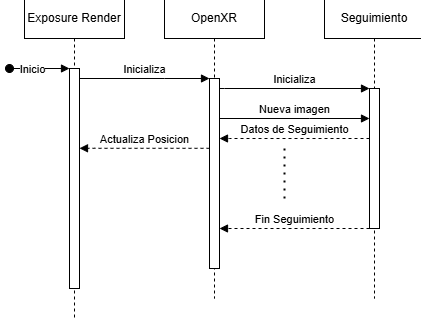
\includegraphics[width=0.75\textwidth]{imaxes/flow_exposure.png}
	\caption{Flujo de integración del seguimiento en Exposure Render.}
	\label{fig:flow_exposure}
\end{figure}

\section{Generación de volúmenes a partir de TC}
Con el fin de facilitar la validación del progreso del proyecto, se utilizó una \acrshort{tc} de pruebas. Dichos datos contienen la sección superior (hombros y cabeza) de un sujeto, mostrado en la \figurename~\ref{fig:manix_full}. Durante el desarrollo se sugirió como posible caso práctico seleccionar el cráneo del sujeto en los datos de prueba y trabajar en la alineación 3D sobre el mismo.

Con el fin de seleccionar una sección concreta para exportar, se utilizaron las herramientas para segmentar volúmenes de 3D Slicer.
Al abrir el programa se pueden ver las vistas, en las que se representará el \acrshort{tc} una vez cargado, como se muestra en la captura de pantalla de la \figurename~\ref{fig:3dslier}.
Se utilizó principalmente la herramienta de «Thresholding» que permite seleccionar partes del modelo cuyas intensidades se comprenden en un intervalo o «threshold» (ver \figurename~\ref{fig:seg_cr}). Posteriormente, para la eliminación de las partes del modelo no deseadas, se utilizó la herramienta de borrado hasta alcanzar el volumen deseado.

\begin{figure}
	\centering
	\begin{subfigure}{.4\textwidth}
		\includegraphics[width=\textwidth]{imaxes/manix_full.png}
		\caption{TC usado en el desarrollo.}\label{fig:manix_full}
	\end{subfigure}
	\begin{minipage}[b]{.47\textwidth}
		\begin{subfigure}{\textwidth}
			\centering
			\includegraphics[width=\textwidth]{imaxes/captura3dslicer_2.png}
			\caption{ Captura de pantalla de 3D Slicer con los datos cargados.}\label{fig:3dslier}
		\end{subfigure}\\
		\begin{subfigure}{\textwidth}
			\centering
			\includegraphics[width=\textwidth]{imaxes/segment_craneo.png}
			\caption{ Captura de pantalla de 3D Slicer del torso una vez aplicado el thresholding.}\label{fig:seg_cr}
		\end{subfigure}
	\end{minipage}
	\caption{\acrshort{tc} de partida y obtención del modelo 3D final con 3D Slicer.}
\end{figure}

\section{Impresión 3D del volumen}
Durante el proceso de segmentación y exportación del modelo, pueden surgir inconsistencias geométricas debido a que el modelo se genera directamente de los datos volumétricos del TC, en lugar de construirse a partir de primitivas geométricas predefinidas. Estas irregularidades, que incluyen superficies no continuas o vértices mal conectados, impedirían un correcto proceso de Slicing y, por consiguiente, la generación adecuada del archivo GCODE necesario para la impresión 3D. Para solucionar este problema, se utilizó el software Meshmixer, una herramienta especializada en la reparación y optimización de mallas 3D. Como se muestra en la \figurename~\ref{fig:arr_geo}, el modelo exportado presenta varios puntos problemáticos, señalados por marcadores, que corresponden a errores geométricos derivados del proceso de exportación. Una vez corregidos estos defectos mediante las herramientas de reparación de Meshmixer, el modelo quedó preparado para su impresión.

\begin{figure}
	\centering
	\includegraphics[width=0.6\textwidth]{imaxes/arreglo_geo.png}
	\caption{Modelo de cráneo 3D con geometrías erróneas.}
	\label{fig:arr_geo}
\end{figure}

Como se comenta en el Capítulo \ref{chap:hs}, para una pieza con una geometría tan compleja, se requeriría una gran cantidad de soportes. Debido a esto, se optó por la impresora Fuse 1 para la impresión de este modelo. A diferencia de una impresora 3D al uso, esta impresora utiliza un láser para fijar capa a capa el polvo de nylon, lo que garantiza una gran resolución en la pieza final y una gran durabilidad de la misma.

Posterior al proceso de impresión es necesario retirar el material sobrante en la cámara de recuperación que cuenta con distintos utensilios para evitar malgastar el material sobrante ya que puede ser reutilizado.

\begin{figure}%
	\centering
	\subfloat[\centering Pieza en el proceso de recuperación del material.]{{\includegraphics[width=.4\textwidth]{imaxes/limpiando_fig.png} }}%
	\qquad
	\subfloat[\centering  Pieza final.]{{\includegraphics[width=.4\textwidth]{imaxes/limpia_fig.png} }}%
	\caption{Proceso de recuperación de material.}%
	\label{fig:limpieza}%
\end{figure}

\section{Desarrollo del marcador fiduciario}
\label{sec:marcador_fiduciario}

\subsection{Planteamiento del problema y selección de la solución}
Obtener la posición y rotación de una figura desconocida en el espacio es uno de los problemas principales a la hora de implementar soluciones de realidad virtual o aumentada, ya que requiere encontrar correspondencias entre objetos conocidos en el espacio y sus proyecciones en el vídeo.

Si bien existen aproximaciones que buscan puntos claves de las figuras o reconocen sus geometrías mediante técnicas de visión artificial e inteligencia artificial, se optó por el uso de  marcadores fiduciarios por varios motivos:

\begin{itemize}
    \item \textbf{Independencia del hardware}: Permite replicar el seguimiento del objeto independientemente del hardware utilizado, ya que una vez calibrada la cámara no se requiere ningún otro tipo de ajuste en el sistema.
    \item \textbf{Robustez frente a oclusiones}: Permite mantener el seguimiento a pesar de que parte del marcador se encuentre ocluido o no esté completamente en el campo de visión de la cámara.
    \item \textbf{Simplicidad de implementación}: Dados los recursos disponibles, se optó por utilizar la librería ArUco para generar y seguir el marcador, aprovechando su madurez y estabilidad.
\end{itemize}

\subsection{Fundamentos teóricos del seguimiento con ArUco}

ArUco a la hora de detectar la posición de un marcador, trabaja con un modelo de coordenadas pin-hole, donde las coordenadas y rotación de los objetos detectados se expresan en función de la posición de la cámara.
El calibrado de la cámara permite determinar la proyección de cualquier punto en las 3 dimensiones del espacio en el sensor de la cámara. En una cámara ideal, un punto 3D $(X, Y, Z)$ en el espacio se proyectaría en el píxel:
\begin{align*}
	x_{ideal} & = \frac{X \cdot fx}{Z} + cx & y_{ideal} = \frac{Y \cdot fy}{Z} + cy
\end{align*}

Sin embargo, las lentes reales introducen distorsiones que deben corregirse. Las coordenadas finales del píxel se calculan aplicando las correcciones de distorsión radial y tangencial:
\begin{align*}
	x_{distorsionada} &= x_{ideal} \cdot (1 + k_1 r^2 + k_2 r^4 + k_3 r^6) + 2p_1 x_{ideal} y_{ideal} + p_2(r^2 + 2x_{ideal}^2) \\
	y_{distorsionada} &= y_{ideal} \cdot (1 + k_1 r^2 + k_2 r^4 + k_3 r^6) + p_1(r^2 + 2y_{ideal}^2) + 2p_2 x_{ideal} y_{ideal}
\end{align*}
donde $r^2 = x_{ideal}^2 + y_{ideal}^2$ es la distancia radial al centro de la imagen.

Donde:
\begin{itemize}
	\item $fx$, $fy$: Es la longitud focal de la lente de la cámara en ambos ejes (píxeles).
	\item $cx$, $cy$: Es el centro óptico del sensor (expresado en píxeles).
	\item $k1$, $k2$, $k3$: Son los coeficientes de distorsión radial que corrigen la curvatura de la lente.
	\item $p1$, $p2$: Son los coeficientes de distorsión tangencial que corrigen la desalineación de la lente.
\end{itemize}
Asumiendo que la ubicación tridimensional del punto con respecto al sistema de referencia de la cámara es conocida. Si se desea conocer la proyección de un punto referido a un sistema de referencia arbitrario, entonces deben mencionarse parámetros extrínsecos. Los parámetros extrínsecos consisten básicamente en las rotaciones tridimensionales (Rvec = {Rx, Ry, Rz}) y las traslaciones tridimensionales (Tvec = {Tx, Ty, Tz}) requeridas para trasladar el sistema de referencia de la cámara al sistema arbitrario. Los elementos de rotación se expresan mediante la fórmula de Rodrigues \cite{mebius2007derivation}, por lo que es posible obtener la matriz de rotación equivalente de 3x3 utilizando la función cv::Rodrigues() de OpenCV.

Cada marcador detectado devuelve como coordenadas la esquina superior izquierda del mismo, o lo que se etiqueta en el ejemplo de la \figurename~\ref{fig:marker_schema} como \emph{corner 0}, en forma de (Rvec = {Rx, Ry, Rz}) como vector de rotación y (Tvec = {Tx, Ty, Tz}) como vector de translación.

\begin{figure}
	\centering
	\includegraphics[width=0.5\textwidth]{imaxes/marker_schema.png}
	\caption{Esquema de un marcador.}
	\label{fig:marker_schema}
\end{figure}

Detectar un solo marcador puede fallar por diferentes razones, como malas condiciones de iluminación, movimiento rápido de la cámara, obstrucciones, etc. Para superar ese problema, ArUco permite el uso de tablas de marcadores como la mostrada en la \figurename~\ref{fig:board_schema}. Cada tabla de marcadores está compuesta por varios marcadores en ubicaciones conocidas. Presentan dos ventajas principales. Primero, dado que hay más de un marcador, es menos probable perderlos todos de vista al mismo tiempo. Segundo, cuanto más marcadores se detecten, más puntos están disponibles para calcular los parámetros extrínsecos de la cámara. Como consecuencia, se obtiene una mayor precisión.

\begin{figure}
	\centering
	\includegraphics[width=0.4\textwidth, angle=90]{imaxes/board_schema.png}
	\caption{Esquema de una tabla de marcadores.}
	\label{fig:board_schema}
\end{figure}

\subsection{Generación de marcadores a partir de diccionarios predefinidos}
El marcador fiduciario utilizado en este proyecto se genera a partir de un diccionario predefinido de ArUco. En la implementación actual se emplea el diccionario \texttt{DICT\_6X6\_250}, que contiene 250 marcadores únicos de 6×6 bits cada uno. Este diccionario fue seleccionado por ofrecer un buen equilibrio entre:

\begin{itemize}
    \item \textbf{Robustez en la detección}: Los marcadores de 6×6 bits proporcionan suficiente información para una detección fiable incluso con cierta degradación de la imagen.
    \item \textbf{Capacidad del diccionario}: Con 250 marcadores únicos disponibles, hay suficientes IDs para implementar múltiples cubos sin conflictos.
    \item \textbf{Replicabilidad}: Al usar un diccionario estándar, los experimentos son fácilmente reproducibles.
\end{itemize}

La generación del cubo marcador sigue un esquema sistemático donde cada cara del cubo contiene una matriz 2×2 de marcadores del mismo diccionario. Los identificadores (IDs) de los marcadores se asignan secuencialmente siguiendo la fórmula:

\begin{center}
\texttt{firstId = cara\_id * 4}\\
\texttt{ids = \{firstId, firstId + 1, firstId + 2, firstId + 3\}}
\end{center}

Donde \texttt{cara\_id} corresponde al número de cara del cubo (0-5). De esta forma:
\begin{itemize}
	\item Cara 0: marcadores con IDs 0, 1, 2, 3
	\item Cara 1: marcadores con IDs 4, 5, 6, 7
	\item Cara 2: marcadores con IDs 8, 9, 10, 11
	\item Cara 3: marcadores con IDs 12, 13, 14, 15
	\item Cara 4: marcadores con IDs 16, 17, 18, 19
	\item Cara 5: marcadores con IDs 20, 21, 22, 23
\end{itemize}

Esta implementación permite utilizar cualquier diccionario predefinido o personalizado de ArUco, siempre y cuando el diccionario contenga al menos 24 marcadores únicos y se respete el orden secuencial de asignación de IDs para cada cara. La modularidad del sistema permite cambiar el diccionario sin necesidad de alterar la lógica de seguimiento del cubo.

\subsection{Algoritmo de cálculo de pose del cubo}
\label{subsec:algoritmo_pose}

El proceso de determinación de la pose del cubo se realiza en varias etapas que transforman las detecciones individuales de cada cara en una pose unificada del centro del cubo.

\subsubsection{Transformación de coordenadas de cara a centro}
Cuando ArUco detecta una cara del cubo, devuelve la posición y orientación correspondientes a la esquina superior izquierda de esa cara (corner 0 en la \figurename~\ref{fig:marker_schema}). Para obtener la pose del centro del cubo, es necesario aplicar una transformación que tenga en cuenta tanto la posición como la orientación actual del marcador.

\subsection{Diseño geométrico del marcador cúbico}

Debido a la versatilidad de las piezas con las que se pretende usar el marcador, se implementó priorizando eliminar las oclusiones del marcador por la pieza. Por este motivo se diseñó como un cubo, de forma que al menos una cara sería visible en todo momento. Se evaluaron otras formas geométricas (prismas rectangulares, pirámides, cilindros), pero estas demostraron menor efectividad de detección con la cámara utilizada en el desarrollo.

El diseño final consiste en un cubo donde cada cara contiene una matriz 2×2 de marcadores del mismo diccionario ArUco. Esta configuración proporciona las siguientes ventajas:

\begin{itemize}
    \item \textbf{Redundancia}: Al tener múltiples marcadores por cara, el sistema puede mantener el tracking incluso si algunos marcadores están ocluidos.
    \item \textbf{Precisión mejorada}: La detección de múltiples marcadores en la misma cara permite calcular la pose con mayor precisión mediante promediado.
    \item \textbf{Robustez}: La forma cúbica garantiza que siempre habrá al menos una cara visible desde cualquier ángulo de observación.
\end{itemize}

Se llevaron a cabo pruebas con distintos diccionarios de marcadores, modificando las tolerancias para los márgenes entre marcadores y los bordes del cubo con el fin de poder mantener unas dimensiones manejables sin comprometer el tamaño de cada marcador individual.
Finalmente, fruto de los tests, se llegó al cubo de la \figurename~\ref{fig:cubo_marker}.

\begin{figure}
	\centering
	\includegraphics[width=0.4\textwidth]{imaxes/cube_layout.png}
	\caption{Layout de las caras del marcador fiduciario.}
	\label{fig:cube_layout}
\end{figure}

\subsection{Transformación de coordenadas de cara a centro del cubo}

El cubo se descompone como se puede ver en la \figurename~\ref{fig:cube_layout}. En un primer momento la detección devuelve la posición y rotación de cada cara de forma individual. Dado que se busca la posición del centro del cubo, sobre cada valor obtenido, se aplica una transformación que tiene en cuenta tanto la posición como la orientación actual del marcador.

Para el cálculo del desplazamiento necesario para cada eje se utiliza la matriz de rotación (obtenida mediante la fórmula de Rodrigues) para asegurar que el desplazamiento se realiza en la dirección correcta respecto a la orientación actual del marcador. Este proceso se aplica para los tres ejes mediante la función \texttt{moveAxis}, cuya implementación detallada se encuentra en el Apéndice~\ref{chap:detalles_implementacion}.

Una vez ajustada la posición del centro, es necesario corregir la orientación de cada cara para mantener un sistema de coordenadas consistente en todo el cubo. Para ello, la función \texttt{cubeCoordinates} aplica las rotaciones necesarias según la cara detectada, usando la cara 0 como referencia. Los detalles completos del código fuente de estas transformaciones de coordenadas están disponibles en el mismo apéndice.

\subsubsection{Fusión de múltiples detecciones}
Cuando se detectan múltiples caras del cubo simultáneamente (hasta 3 caras pueden ser visibles en una sola imagen), el sistema debe combinar las estimaciones individuales para obtener una pose más precisa y estable. El algoritmo implementado utiliza un promediado simple de los vectores de traslación y rotación.

El promediado de vectores de rotación requiere especial atención debido a la naturaleza circular de las rotaciones y posibles discontinuidades en la representación de Rodrigues. El sistema implementa verificaciones para evitar promediar rotaciones que difieran significativamente, lo que podría indicar detecciones erróneas o ambigüedades en la orientación.


\begin{figure}%
	\centering
	\subfloat[\centering Modelo del marcador fiduciario.]{{\includegraphics[width=6cm]{imaxes/cubo_marker.png} }}%
	\qquad
	\subfloat[\centering  Impresión del marcador fiduciario.]{{\includegraphics[width=6cm]{imaxes/cubo_marker_imp.png} }}%
	\caption{Diseño final del marcador fiduciario.}%
	\label{fig:cubo_marker}%
\end{figure}

En caso de que únicamente se detectase una cara del cubo, los vectores de rotación y translación finales serían los obtenidos llegados a este punto. Como se observa en la \figurename~\ref{fig:cubo_detected}, es posible detectar hasta 3 caras simultáneamente en una única imagen, lo que permite aplicar el algoritmo de fusión descrito anteriormente para obtener una estimación más robusta de la pose.

\begin{figure}%
	\centering
	\subfloat[\centering Ejemplo de detección del cubo.]{{\includegraphics[width=6cm]{imaxes/cube_detected.png} }}%
	\qquad
	\subfloat[\centering Ejemplo de detección del cubo con oclusión.]{{\includegraphics[width=6cm]{imaxes/cube_detected_ocluded.png} }}%
	\caption{Imágenes sobre las que se estima la pose del cubo.}%
	\label{fig:cubo_detected}%
\end{figure}

\subsubsection{Procesamiento de secuencias de vídeo}
Hasta ahora, se ha descrito el comportamiento de la aplicación para una única imagen. El procesamiento de secuencias de vídeo consiste en aplicar iterativamente este algoritmo a cada frame de la secuencia. Una vez obtenidos los valores de pose para un frame, el sistema espera al siguiente frame y ejecuta nuevamente el pipeline de detección.

El diagrama muestra claramente las etapas principales del proceso implementado:
\begin{enumerate}
    \item \textbf{Inicialización del sistema}: Apertura de la cámara, carga de parámetros de calibración, creación de las tablas de marcadores para cada cara del cubo e inicialización del detector ArUco.
    \item \textbf{Captura de frame}: Obtención del frame de vídeo desde la cámara.
    \item \textbf{Detección de marcadores}: Identificación inicial de marcadores ArUco en la imagen.
    \item \textbf{Refinamiento de detección}: Mejora de la precisión de detección aplicando el refinamiento específico para cada tabla de marcadores del cubo.
    \item \textbf{Procesamiento por cara}: Para cada una de las seis caras del cubo, se calculan las correspondencias entre puntos de imagen y puntos del objeto 3D.
    \item \textbf{Cálculo de pose individual}: Estimación de pose mediante solvePnP para cada cara que tenga correspondencias válidas.
    \item \textbf{Transformación al centro}: Conversión de las coordenadas de cada cara al centro del cubo utilizando las transformaciones geométricas correspondientes.
    \item \textbf{Promediado de poses}: Combinación de todas las poses válidas obtenidas para generar una estimación final más robusta.
    \item \textbf{Comunicación de resultados}: Retorno de la pose final calculada o pose vacía si no se detectaron marcadores.
\end{enumerate}

El diagrama de flujo completo del algoritmo, desde la captura de imagen hasta la obtención de la pose final del cubo, se puede consultar en el Apéndice~\ref{chap:diagramas_detallados}.

\section{Implementación del Passthrough en Exposure Render}
\subsection{Captura de imagen}
\label{subsec:captura_imagen}
En un primer momento para la obtención de imágenes sobre las que poder realizar el seguimiento del marcador fiduciario se pretendían usar las propias cámaras frontales del HTC Vive Pro 2. Se trata de un par de cámaras colocadas longitudinalmente a lo largo del frontal del casco, que permiten su uso en aplicaciones de realidad aumentada y realidad mixta.
Se trató de acceder a las mismas mediante el uso de SRworks C++ SDK y con librerías de terceros a pesar de no tener éxito. Posteriormente tras conversaciones con el equipo de soporte se concluyó que no era posible el acceso a las cámaras de forma nativa. Solo a través de Unreal Engine o Unity en su defecto, lo que nos hizo descartar esta posibilidad. Cabe destacar que durante el desarrollo del proyecto HTC retiró el soporte de la extensión de passthrough en OpenXR, por lo que versiones posteriores del runtime dejaron de anunciar esta funcionalidad a través de la API de extensiones de OpenXR.
La alternativa era acceder a las imágenes a través de una cámara de terceros. Esta opción presentaba la desventaja de imposibilitar el tratamiento de la imagen directamente en GPU, pero era la única viable dentro del contexto del TFG.

\subsection{Integración del seguimiento}
Con el fin de no aumentar la cantidad de dependencias de un proyecto de la envergadura de Exposure Render, se trató de implementar la solución de tracking como una librería independiente que se pudiese integrar en el proyecto.

La integración del sistema de tracking ArUco en Exposure Render se realizó como una librería independiente que proporciona la funcionalidad de seguimiento de marcadores fiduciarios. El punto central de esta integración es la función \texttt{getCubePoseMatrix}, que actúa como interfaz principal entre el sistema de tracking y la aplicación de realidad aumentada.

\subsubsection{Función getCubePoseMatrix}
La función \texttt{getCubePoseMatrix} es la interfaz principal que proporciona la pose del cubo marcador en el espacio tridimensional. Los parámetros de esta función incluyen configuraciones para visualización, dimensiones físicas del marcador, rutas de calibración y directorios de configuración.

Los detalles completos de la signatura de esta función y sus parámetros se pueden consultar en el Apéndice~\ref{chap:detalles_implementacion}.

\subsubsection{Implementación como hilo independiente}
Para minimizar la latencia y mantener la fluidez del renderizado principal, el sistema de tracking se implementó como un hilo independiente mediante la clase \texttt{Tracking} que encapsula toda la funcionalidad de seguimiento.

El flujo de ejecución del tracking opera en un hilo separado (\texttt{poseThread}) que ejecuta continuamente el siguiente proceso:

\begin{enumerate}
    \item \textbf{Captura de pose del headset}: Obtiene la matriz de transformación actual del casco VR desde el sistema OpenXR.
    \item \textbf{Captura de imagen}: Adquiere una nueva imagen desde la cámara del sistema.
    \item \textbf{Procesamiento de marcadores}: Ejecuta la detección y seguimiento de marcadores ArUco llamando a \texttt{getCubePoseMatrix}.
    \item \textbf{Sincronización de datos}: Actualiza de forma thread-safe la pose más reciente del cubo y la imagen procesada.
    \item \textbf{Actualización del overlay}: Envía la imagen procesada al sistema de overlay para visualización en realidad aumentada.
\end{enumerate}

La gestión de concurrencia utiliza mecanismos de sincronización para garantizar la integridad de los datos compartidos:
\begin{itemize}
    \item \textbf{std::mutex}: Protege el acceso a las variables \texttt{\_latestPose} y \texttt{\_latestCameraImage}.
    \item \textbf{std::atomic<bool>}: Controla el estado de ejecución del hilo mediante \texttt{\_poseThreadRunning}.
    \item \textbf{Lock guards}: Garantizan el acceso exclusivo durante las operaciones de lectura y escritura de datos compartidos.
\end{itemize}

Esta arquitectura asegura que el hilo principal de renderizado no se vea bloqueado por las operaciones de procesamiento de imagen, manteniendo una alta tasa de refresco en la experiencia de realidad aumentada mientras proporciona datos de tracking actualizados de forma continua.

\subsubsection{Estructura de datos PoseMatrix4x4 y transformaciones de coordenadas}

Para facilitar la integración con Exposure Render, la librería de tracking utiliza la estructura \texttt{PoseMatrix4x4}, que representa una matriz de 4×4. Esta estructura encapsula tanto la rotación como la traslación del marcador en el espacio 3D.

La función \texttt{getCubePoseMatrix} implementa una serie de transformaciones para que la pose del cubo detectada por ArUco sea directamente utilizable por el motor de renderizado de Exposure Render. El proceso incluye:

\begin{enumerate}
    \item \textbf{Construcción de la matriz de transformación}: Conversión de vectores de rotación y traslación de ArUco a matriz de transformación 4×4 que representa la pose del marcador en el sistema de coordenadas de la cámara.
    \item \textbf{Inversión para obtener la transformación del mundo al marcador}: La matriz de ArUco representa la transformación del marcador a la cámara, por lo que se invierte para obtener la transformación que posiciona objetos virtuales respecto al marcador detectado.
    \item \textbf{Conversión de sistemas de coordenadas}: Compatibilización entre el orden row-major de OpenCV y column-major de OSG.
\end{enumerate}

Los detalles matemáticos completos de estas transformaciones, incluyendo el código de implementación y las ecuaciones específicas, se pueden consultar en el Apéndice~\ref{chap:detalles_implementacion}.




\paragraph{Transformación al \gls{worldspace}}
Finalmente, la pose del cubo se transforma desde el espacio de coordenadas de la cámara al \gls{worldspace} del entorno VR. Esta transformación se realiza mediante la multiplicación de la matriz del cubo por la matriz de transformación del headset VR, que se obtiene del sistema OpenXR:

\begin{lstlisting}[language=C++]
cv::Mat headsetMat = poseMatrixToCvMat(headsetPose);
finalTransform = headsetMat * cubeModelTransposed;
\end{lstlisting}

La transformación completa se puede expresar matemáticamente como una cadena de operaciones matriciales:

$$\mathbf{T}_{world} = \mathbf{H} \cdot (\mathbf{T}_{ArUco}^{-1})^T$$

Donde:
\begin{itemize}
    \item $\mathbf{T}_{world}$: Matriz de transformación final del cubo en el \gls{worldspace}
    \item $\mathbf{H}$: Matriz de transformación del headset VR en el \gls{worldspace} (obtenida de OpenXR)
    \item $\mathbf{T}_{ArUco}$: Matriz de transformación vista del cubo detectada por ArUco (de cubo a cámara)
    \item $(\mathbf{T}_{ArUco}^{-1})^T$: Matriz transpuesta de la inversa de $\mathbf{T}_{ArUco}$ (modelo del cubo en espacio de cámara)
\end{itemize}

Esta cadena de transformaciones convierte la pose detectada por ArUco desde el espacio de coordenadas de la cámara al \gls{worldspace} compatible con Exposure Render.

Este enfoque permite que el objeto virtual renderizado por Exposure Render se mantenga perfectamente alineado con el marcador físico en el mundo real, independientemente de los movimientos del usuario y la cámara. La secuencia completa de transformaciones asegura que las convenciones de coordenadas de ArUco, OpenCV, \acrshort{osg} y OpenXR sean compatibles entre sí, proporcionando una experiencia de realidad aumentada coherente y precisa.

\subsection{Consideraciones de implementación alternativa}

Durante el desarrollo del proyecto, surgieron limitaciones técnicas en la integración completa con Exposure Render que condujeron a la exploración de enfoques alternativos de visualización. Estas limitaciones incluyeron incompatibilidades organizativas en cuanto al acceso al \acrshort{hmd} y complejidades en la transformación entre los sistemas de \gls{tracking} y renderizado, entre otros.

Como resultado de estas consideraciones técnicas, se desarrolló una implementación de renderizado independiente que permitió validar la funcionalidad del sistema de seguimiento de marcadores y demostrar la viabilidad del enfoque propuesto. Esta solución alternativa mantuvo los principios fundamentales de seguimiento en tiempo real, proporcionando una base sólida para futuras integraciones con sistemas de renderizado más complejos.

\section{Aplicación Independiente de Realidad Aumentada}
\label{sec:aplicacion_independiente}

Con el fin de demostrar la viabilidad del sistema de \gls{tracking} desarrollado y proporcionar una herramienta práctica para la visualización de modelos anatómicos sobre marcadores fiduciarios, se implementó una aplicación independiente de realidad aumentada. Esta aplicación combina las capacidades de seguimiento ArUco desarrolladas anteriormente con un sistema de renderizado 3D que permite cargar y visualizar modelos anatómicos de diversas fuentes.

\subsection{Arquitectura de la aplicación}

La aplicación se estructura en varios módulos funcionales que operan de manera coordinada:

\begin{itemize}
    \item \textbf{Módulo de captura}: Gestiona la adquisición de imágenes desde la cámara web y la inicialización de los parámetros de calibración.
    \item \textbf{Módulo de tracking}: Utiliza la librería de seguimiento ArUco desarrollada para detectar y seguir el marcador cúbico en tiempo real.
    \item \textbf{Módulo de renderizado}: Implementa el sistema de visualización 3D utilizando \acrshort{glfw}, \acrshort{glew} y \acrshort{glm} para el renderizado con OpenGL.
    \item \textbf{Módulo de carga de modelos}: Integra \acrshort{assimp} para soportar múltiples formatos de archivo 3D (FBX, OBJ, STL, etc.).
\end{itemize}

El punto de entrada principal de la aplicación coordina la ejecución de todos los módulos mediante hilos independientes para garantizar un rendimiento óptimo.

\subsection{Sistema de renderizado basado en OpenGL}

El sistema de renderizado implementado utiliza OpenGL con shaders programables para proporcionar capacidades de visualización 3D avanzadas.

El renderizador OpenGL proporciona las siguientes características:

\begin{itemize}
    \item \textbf{Modelo de iluminación}: Implementa un \gls{phong} con componentes ambiente, difusa y especular.
    \item \textbf{Soporte para texturas}: Permite aplicar texturas a los modelos cuando están disponibles en el archivo del modelo.
    \item \textbf{Renderizado fuera de pantalla}: Utiliza framebuffers para renderizar la escena en una textura que posteriormente se compone con la imagen de la cámara.
    \item \textbf{Compatibilidad con múltiples formatos}: Mediante \acrshort{assimp}, soporta formatos como FBX, OBJ, 3DS, COLLADA, etc.
\end{itemize}

El pipeline de renderizado se basa en dos tipos de shaders principales que operan en diferentes etapas del proceso de renderizado:

\subsubsection{Vertex Shader}
El vertex shader se encarga de procesar cada vértice individual del modelo 3D. Su función principal es transformar las coordenadas de los vértices desde el espacio del modelo al espacio de pantalla mediante la aplicación de las matrices de transformación (modelo, vista y proyección). Además, prepara la información necesaria para el fragment shader, incluyendo las posiciones transformadas en el espacio mundial, las normales corregidas para la iluminación y las coordenadas de textura.

\subsubsection{Fragment Shader}
El fragment shader opera sobre cada píxel de las superficies renderizadas e implementa el \gls{phong} para calcular la iluminación final. Este shader combina tres componentes de iluminación: la luz ambiente (que proporciona una iluminación base uniforme), la luz difusa (que simula la \gls{lambert} dependiente del ángulo de incidencia) y la luz especular (que genera los brillos característicos de las superficies). El resultado final se combina con las texturas del modelo cuando están disponibles, proporcionando una apariencia adecuada.

\subsection{Sistema de carga de modelos}

La aplicación implementa un sistema de carga de modelos basado en la librería \acrshort{assimp}, que permite trabajar con múltiples formatos de archivo 3D de manera unificada. El sistema aprovecha las capacidades de \acrshort{assimp} para procesar automáticamente la geometría del modelo y convertirla en estructuras de datos optimizadas para el renderizado en tiempo real.

El proceso de carga se estructura en tres etapas principales. En primer lugar, se inicializa el importador de \acrshort{assimp} con flags de post-procesamiento específicos que garantizan la compatibilidad con el pipeline de renderizado:

\begin{lstlisting}[language=C++]
Assimp::Importer importer;
const aiScene* scene = importer.ReadFile(filename, 
    aiProcess_Triangulate | aiProcess_GenNormals | aiProcess_FlipUVs);
\end{lstlisting}

Estos flags aseguran que todos los polígonos del modelo estén triangulados, que las normales se generen automáticamente si no están presentes en el archivo original, y que las coordenadas de textura estén orientadas correctamente para el sistema de coordenadas de OpenGL.

En la segunda etapa, se valida la estructura del archivo cargado y se extrae la primera malla disponible en la escena. \acrshort{assimp} organiza los modelos en una jerarquía de nodos que pueden contener múltiples mallas, pero para simplificar la implementación se procesa únicamente la primera malla encontrada.

Finalmente, se iteran los vértices de la malla para extraer las posiciones, normales y coordenadas de textura, almacenándolas en vectores que posteriormente serán transferidos a la GPU:

\begin{lstlisting}[language=C++]
for (unsigned int i = 0; i < ai_mesh->mNumVertices; ++i) {
    mesh.vertices.push_back(ai_mesh->mVertices[i]);
    mesh.normals.push_back(ai_mesh->mNormals[i]);
    mesh.texCoords.push_back(ai_mesh->mTextureCoords[0][i]);
}
\end{lstlisting}

Este enfoque permite cargar modelos anatómicos complejos procedentes de software de segmentación médica como 3D Slicer, así como modelos creados en aplicaciones de modelado 3D estándar, proporcionando flexibilidad en las fuentes de datos sin comprometer el rendimiento del sistema de renderizado.

\subsection{Flujo de ejecución de la aplicación}

El flujo principal de la aplicación coordina todos los componentes del sistema:

\begin{enumerate}
    \item \textbf{Inicialización de rutas}: Se establecen las rutas a los archivos de calibración, marcadores y modelos 3D.
    \item \textbf{Creación del hilo de captura}: Se inicia un hilo independiente para el \gls{tracking} de marcadores mediante \texttt{captureThreadFunc}.
    \item \textbf{Inicialización del renderizador}: Se crea e inicializa el sistema de renderizado (OpenGL o OpenCV según la configuración).
    \item \textbf{Bucle principal de renderizado}: Se ejecuta el bucle principal que combina las imágenes de la cámara con los modelos 3D renderizados.
\end{enumerate}

\begin{lstlisting}[language=C++]
int main()
{
    // Configuración de parámetros del proyecto
    std::string calibrationPath = getCalibrationPath();
    std::string markersPath = getMarkersPath();
    std::string modelsPath = getModelsPath();
    
    // Inicialización del hilo de tracking
    std::thread captureThread(captureThreadFunc, 
        true,  // showVisualization
        markerSideLength, 
        markerGapLength,
        calibrationPath,
        markersPath);
    
    // Inicialización del renderizador
    if (!initializeRenderer(cameraResolution, modelsPath)) {
        std::cerr << "Error: Failed to initialize renderer" << std::endl;
        return -1;
    }
    
    // Bucle principal de renderizado
    while (!shouldClose()) {
        Mat renderedFrame = renderFrame(pose, cameraImage);
        
        if (!renderedFrame.empty()) {
            displayFrame(renderedFrame);
        }
        
        processEvents();
    }
    
    return 0;
}
\end{lstlisting}

Esta arquitectura modular permite que la aplicación funcione como una herramienta independiente y versátil para la visualización de modelos 3D en realidad aumentada. El diseño implementado demuestra la efectividad del sistema de \gls{tracking} desarrollado y proporciona una base sólida para futuras extensiones y mejoras. La separación en módulos independientes facilita la integración con otros sistemas de renderizado y permite adaptar la solución a diferentes casos de uso manteniendo la robustez del seguimiento de marcadores.


\chapter{Conclusiones y trabajo futuro}\label{chap:c}
\lettrine{C}{omo} cierre del trabajo, cabe reflexionar sobre el desarrollo del mismo así como sobre su estado actual, y su futuro. Dado por finalizado el trabajo, se han alcanzado buena parte de los objetivos fijados en su concepción:

\begin{itemize}
	\item Se identificaron métodos para la extracción de secciones de \acrshort{tc} así como para el refinado de las mismas. También se analizaron las posibilidades de impresión optimizando el uso de los materiales y de las capacidades de las impresoras. Esto ha permitido trabajar sobre piezas en un nivel más visual e interactivo.
	\item Se ha llevado a cabo un estudio de las soluciones existentes para el seguimiento 3D realizando pruebas de las mismas sobre los datos propios para extraer las ventajas y desventajas de cada solución en un nivel práctico.
	\item Se han diseñado e impreso una gran cantidad de marcadores fiduciarios sobre los que se han realizado pruebas de forma iterativa con el fin de refinar y optimizar el diseño hasta obtener un resultado que satisface las características del proyecto. Todo esto mediante el uso de software libre creando así un proceso adaptable a otros casos de uso.
	\item Se desarrolló un sistema robusto de seguimiento de marcadores cúbicos basado en ARuco que permite detectar hasta 3 caras simultáneamente, proporcionando mayor precisión y resistencia a oclusiones parciales.
	\item Se implementó un algoritmo de transformación de coordenadas que permite convertir las poses detectadas por ARuco en matrices de transformación compatibles con sistemas de renderizado 3D, resolviendo las incompatibilidades entre diferentes convenciones de coordenadas.
	\item Se creó una aplicación independiente de realidad aumentada que demuestra la viabilidad del sistema de tracking desarrollado, integrando capacidades de carga de modelos 3D mediante \acrshort{assimp} y renderizado con iluminación \gls{phong}.
	\item Se estableció una arquitectura modular que permite la integración del sistema de tracking como librería independiente, facilitando su incorporación en proyectos existentes como Exposure Render.
	\item Se ha integrado parcialmente la solución en el proyecto de \citeauthor{IglesiasGuitian2022}, sentando las bases para una integración completa que desvirtualice casos de uso médicos reales.
\end{itemize}
\subsection{Enriquecimiento Formativo}
Es imprescindible destacar la vertiente formativa que presenta este trabajo dada su naturaleza como trabajo de fin de grado. El autor ha tenido la posibilidad de trabajar sobre una serie de campos de lo mas variados que comprenden la imagen médica, la impresión 3D, la visión artificial, la realidad virtual y el renderizado en un motor de trazado de rayos entr otros. Por otra parte, mencionar la exposición a un ambiente investigador en el \acrshort{citic} del que poder empaparse de la forma de trabajar y la cooperación entre iguales. También se trató de una primera puesta en práctica de los conceptos aprendidos sobre la gestión de proyectos que resultó enriquecedora.
\subsection{Trabajo futuro}
En la actualidad el proyecto tiene distintas vertientes que pueden ser desarrolladas en el futuro:

\subsubsection{Integración completa con Exposure Render}
Una de las líneas de trabajo más prometedoras consiste en completar de forma exitosa la integración del sistema de tracking con Exposure Render. Aunque se han establecido las bases arquitectónicas y se ha desarrollado la librería de tracking como módulo independiente, quedan aspectos por resolver relacionados con el acceso nativo a las cámaras del HTC Vive Pro 2 y la optimización del pipeline de transformación de coordenadas. La consecución de esta integración permitiría aprovechar las capacidades avanzadas de renderizado volumétrico de Exposure Render para visualizar modelos anatómicos extraídos de TC con calidad fotorrealista en tiempo real.

\subsubsection{Desarrollo de benchmarks para evaluación de marcadores}
Sería valioso desarrollar un sistema de benchmarking que permita evaluar objetivamente la efectividad de distintos tipos de marcadores fiduciarios en diferentes condiciones. Este benchmark incluiría métricas como precisión de detección, robustez frente a oclusiones, estabilidad del tracking en movimiento y rendimiento bajo diferentes condiciones de iluminación. Los resultados permitirían optimizar el diseño de marcadores para casos de uso específicos y proporcionarían una base científica para futuras investigaciones en el campo.

\subsubsection{Implementación de filtrado de Kalman}
Si bien el sistema actual de seguimiento es completamente funcional, en sistemas donde la tasa de refresco de la cámara no es suficientemente alta, el seguimiento puede dar una sensación de escalonado. Una posible solución sería implementar un filtro de Kalman que, bien configurado, ayudaría a estimar pasos intermedios entre imágenes y a reducir el ruido en las mediciones de pose. Esto proporcionaría una experiencia más fluida y permitiría mantener el tracking incluso en frames donde el marcador no sea detectado temporalmente \cite{welch2020kalman}.

\subsubsection{Mejoras en realidad aumentada mediante fusión de cámaras}
Una segunda vertiente de mejora consistiría en reconstruir sobre las imágenes extraídas del casco un ambiente de realidad aumentada más robusto. Esto incluiría utilizar las imágenes de ambas cámaras del HTC Vive Pro 2 para crear una imagen compuesta estereoscópica que permita una mejor detección del marcador fiduciario y una experiencia de realidad aumentada más inmersiva. Aprovechándose de los desarrollos de la interfaz de realidad virtual del proyecto de \citeauthor{IglesiasGuitian2022}, se podría trabajar con la pieza virtual modificando sus parámetros visuales en tiempo real.

\subsubsection{Extensión a múltiples marcadores}
Finalmente, otra línea de desarrollo interesante sería la extensión del sistema para soportar el seguimiento simultáneo de múltiples marcadores cúbicos independientes. Esto permitiría el seguimiento de varios objetos anatómicos simultáneamente o la implementación de sistemas de referencia más complejos que mejoren la precisión general del tracking mediante triangulación entre marcadores.

%%%%%%%%%%%%%%%%%%%%%%%%%%%%%%%%%%%%%%%%
% Apéndices, glosarios e bibliografía  %
%%%%%%%%%%%%%%%%%%%%%%%%%%%%%%%%%%%%%%%%

\appendix
\appendixpage
\chapter{Detalles de Implementación}
\label{chap:detalles_implementacion}

\lettrine{E}{n} este apéndice se incluyen los detalles técnicos de implementación del sistema de tracking, incluyendo el código fuente completo de las funciones principales y los algoritmos de transformación de coordenadas.

\section{Implementación del algoritmo de tracking}

\subsection{Función moveAxis}
La función \texttt{moveAxis} permite desplazar la pose del marcador a lo largo de un eje específico del sistema de coordenadas del cubo:

\begin{lstlisting}[language=C++]
cv::Vec3d moveAxis(cv::Vec3d tvec, cv::Vec3d rvec, double distance, int axis)
{
    cv::Mat rotationMatrix;
    cv::Mat rotationMatrixTransposed;
    Rodrigues(rvec, rotationMatrix);
    rotationMatrixTransposed = rotationMatrix.t();
    double* rz = rotationMatrixTransposed.ptr<double>(axis); // x=0, y=1, z=2
    tvec[0] -= rz[0] * distance;
    tvec[1] -= rz[1] * distance;
    tvec[2] -= rz[2] * distance;
    return tvec;
}
\end{lstlisting}

\subsection{Aplicación de las transformaciones al centro del cubo}
El siguiente código muestra cómo se aplican las transformaciones para mover la pose desde la esquina del marcador hasta el centro del cubo:

\begin{lstlisting}[language=C++]
tvecs = moveAxis(tvecs, rvecs, -SIDELENGTH, 0);
tvecs = moveAxis(tvecs, rvecs, -SIDELENGTH, 1);
tvecs = moveAxis(tvecs, rvecs, -SIDELENGTH, 2);
\end{lstlisting}

\subsection{Función cubeCoordinates}
La función \texttt{cubeCoordinates} aplica las rotaciones necesarias según la cara detectada, usando la cara 0 como referencia:

\begin{lstlisting}[language=C++]
void cubeCoordinates(int id, cv::Vec3d& rvecs, cv::Vec3d& tvecs, float sideLength)
{
    tvecs = moveAxis(tvecs, rvecs, -SIDELENGTH, 0);
    tvecs = moveAxis(tvecs, rvecs, -SIDELENGTH, 1);
    tvecs = moveAxis(tvecs, rvecs, -SIDELENGTH, 2);
    switch (id)
    {
    case 1://cara 1
        rvecs = rotateXAxis(rvecs, -M_PI / 2);
        break;
    case 2://cara 2
        rvecs = rotateXAxis(rvecs, M_PI);
        break;
    case 3://cara 3
        rvecs = rotateYAxis(rvecs, M_PI / 2);
        rvecs = rotateZAxis(rvecs, M_PI);
        break;
    case 4://cara 4
        rvecs = rotateXAxis(rvecs, M_PI);
        rvecs = rotateYAxis(rvecs, -M_PI / 2);
        break;
    case 5://cara 5
        rvecs = rotateXAxis(rvecs, M_PI / 2);
        break;
    default://La cara 0 no precisa rotar
        break;
    }
}
\end{lstlisting}

\section{Transformaciones de coordenadas entre sistemas}

\subsection{Conversión del espacio de cámara al espacio del cubo}
ARuco proporciona la pose del marcador como vectores de rotación y traslación que se convierten en una matriz de transformación 4×4:

\begin{lstlisting}[language=C++]
cv::Mat cubeTransform = buildTransformation(rvecFinal, tvecFinal);
\end{lstlisting}

\subsection{Inversión para obtener la matriz modelo}
Para obtener la pose del cubo en el espacio de coordenadas de la cámara:

\begin{lstlisting}[language=C++]
cv::Mat cubeModel;
cv::invert(cubeTransform, cubeModel);
\end{lstlisting}

\subsection{Conversión entre sistemas row-major y column-major}
Para compatibilizar OpenCV (row-major) con OSG (column-major):

\begin{lstlisting}[language=C++]
cv::Mat cubeModelTransposed;
cv::transpose(cubeModel, cubeModelTransposed);
\end{lstlisting}

\section{Interfaz principal de tracking}

\subsection{Función getCubePoseMatrix}
La función principal que proporciona la pose del cubo marcador:

\begin{lstlisting}[language=C++]
PoseMatrix4x4 getCubePoseMatrix(
    bool showVisualization,
    double markerSideLength,
    double markerGapLength,
    const std::string& calibrationFilePath,
    const std::string& boardDirPath,
    ImageData& undistortedImage);
\end{lstlisting}

Esta función encapsula toda la funcionalidad de tracking y actúa como interfaz principal entre el sistema de seguimiento y la aplicación de realidad aumentada.

\chapter{Capturas de la aplicación en funcionamiento}
\label{chap:capturas}

\lettrine{E}{ste} apéndice presenta una serie de capturas que documentan el funcionamiento de la aplicación de realidad aumentada desarrollada bajo diferentes condiciones de operación. Las imágenes muestran el pipeline completo de procesamiento, desde la captura original de la cámara hasta el renderizado final del modelo 3D.

\section{Escenario sin obstrucciones}
\label{sec:unobstructed}

En este escenario el marcador cúbico se encuentra completamente visible y orientado de forma frontal respecto a la cámara. Este caso representa las condiciones ideales de funcionamiento del sistema.

\begin{figure}[H]
	\centering
	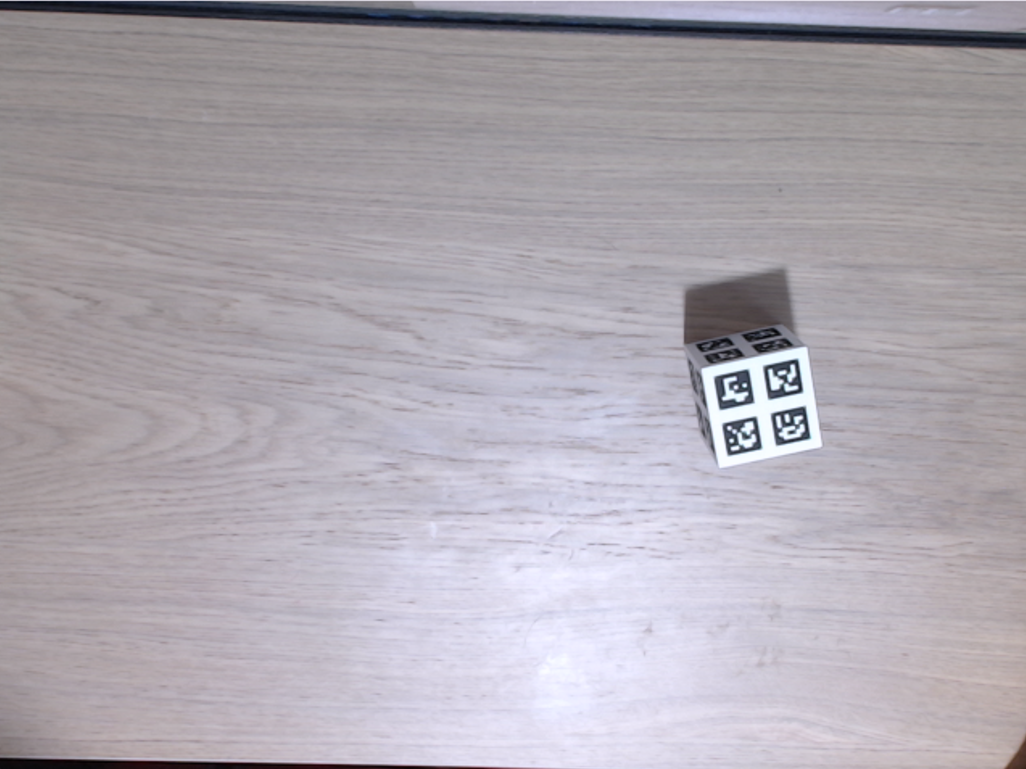
\includegraphics[width=0.8\textwidth]{imaxes/unobstructed_raw_image.png}
	\caption{Imagen original.}
	\label{fig:unobstructed_raw}
\end{figure}

\begin{figure}[H]
	\centering
	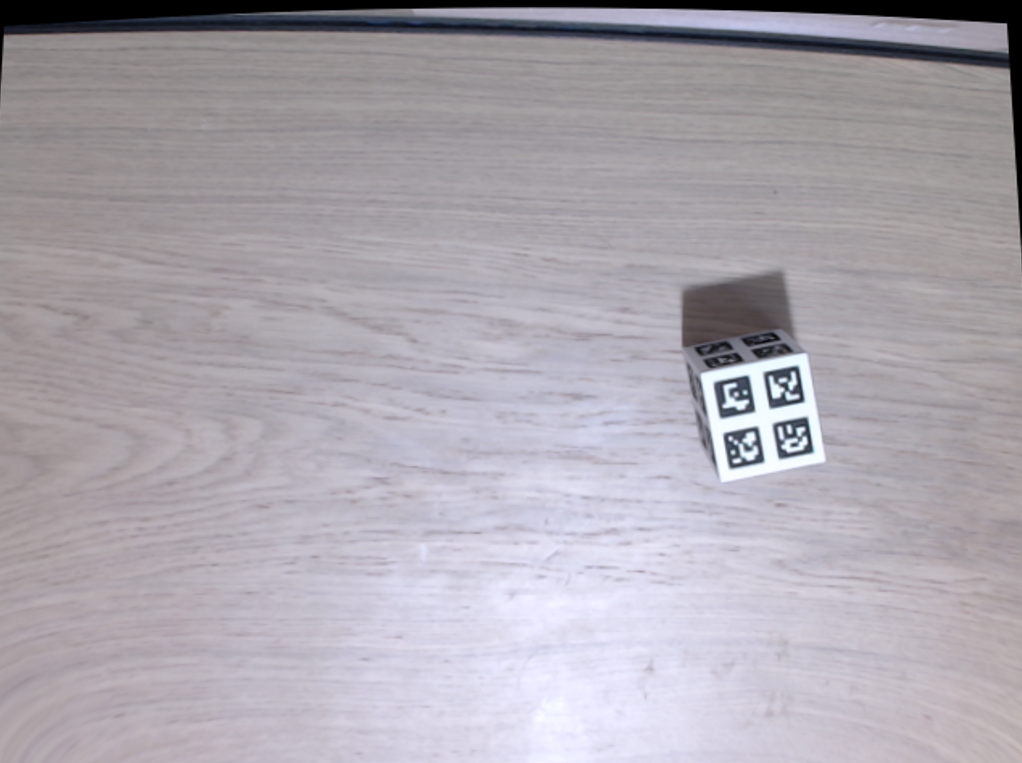
\includegraphics[width=0.8\textwidth]{imaxes/unobstructed_undistorted.png}
	\caption{Imagen corregida tras aplicar la corrección de distorsión de la cámara.}
	\label{fig:unobstructed_undistorted}
\end{figure}

\begin{figure}[H]
	\centering
	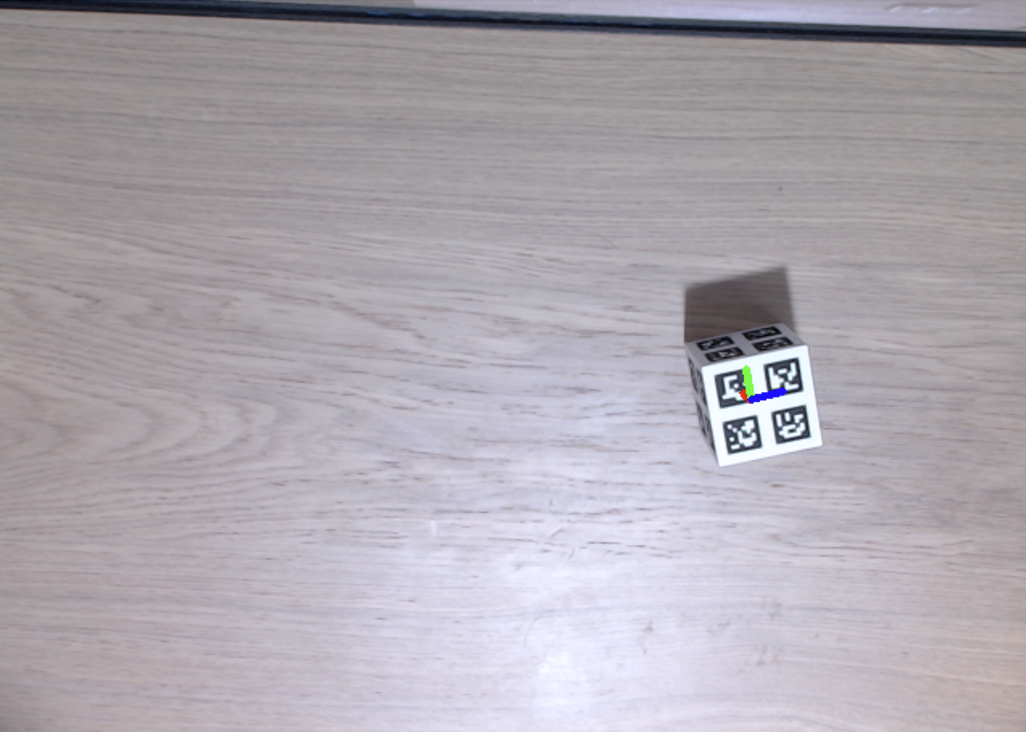
\includegraphics[width=0.8\textwidth]{imaxes/unobstructed_cube_axis.png}
	\caption{Visualización de los ejes de coordenadas sobre el marcador detectado.}
	\label{fig:unobstructed_axes}
\end{figure}

\begin{figure}[H]
	\centering
	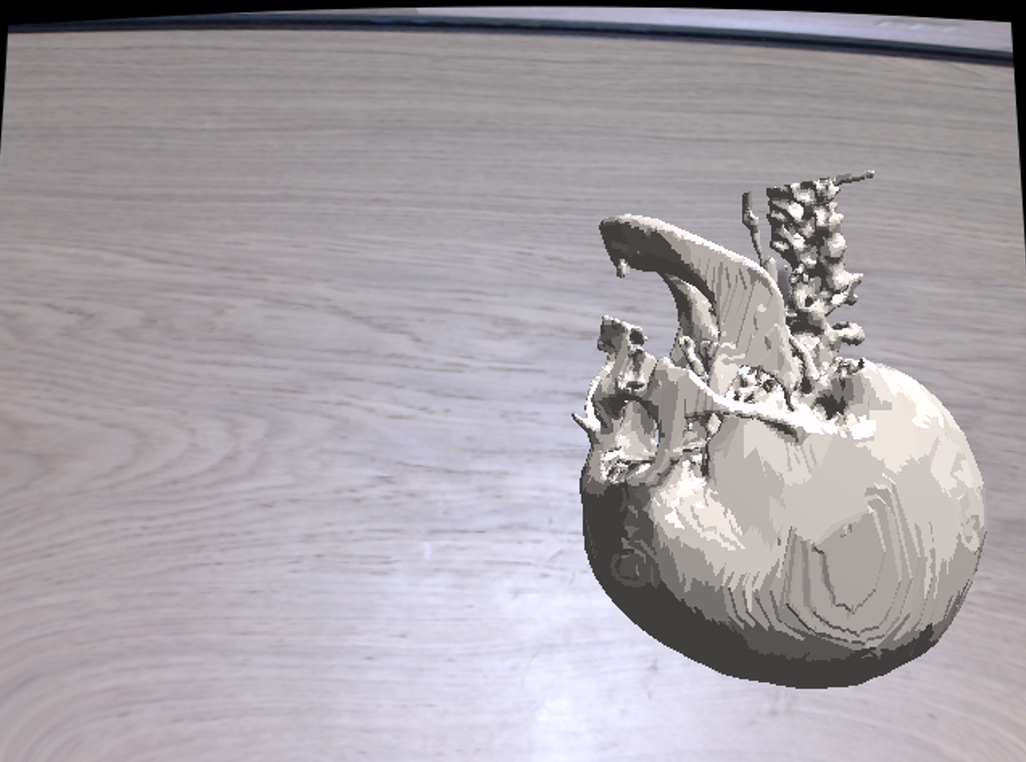
\includegraphics[width=0.8\textwidth]{imaxes/unobstructed_opengl_render.png}
	\caption{Renderizado final del modelo 3D.}
	\label{fig:unobstructed_render}
\end{figure}

\section{Escenario con inclinación}
\label{sec:tilted}

Este escenario evalúa el comportamiento del sistema cuando varias caras del marcador son detectadas.

\begin{figure}[H]
	\centering
	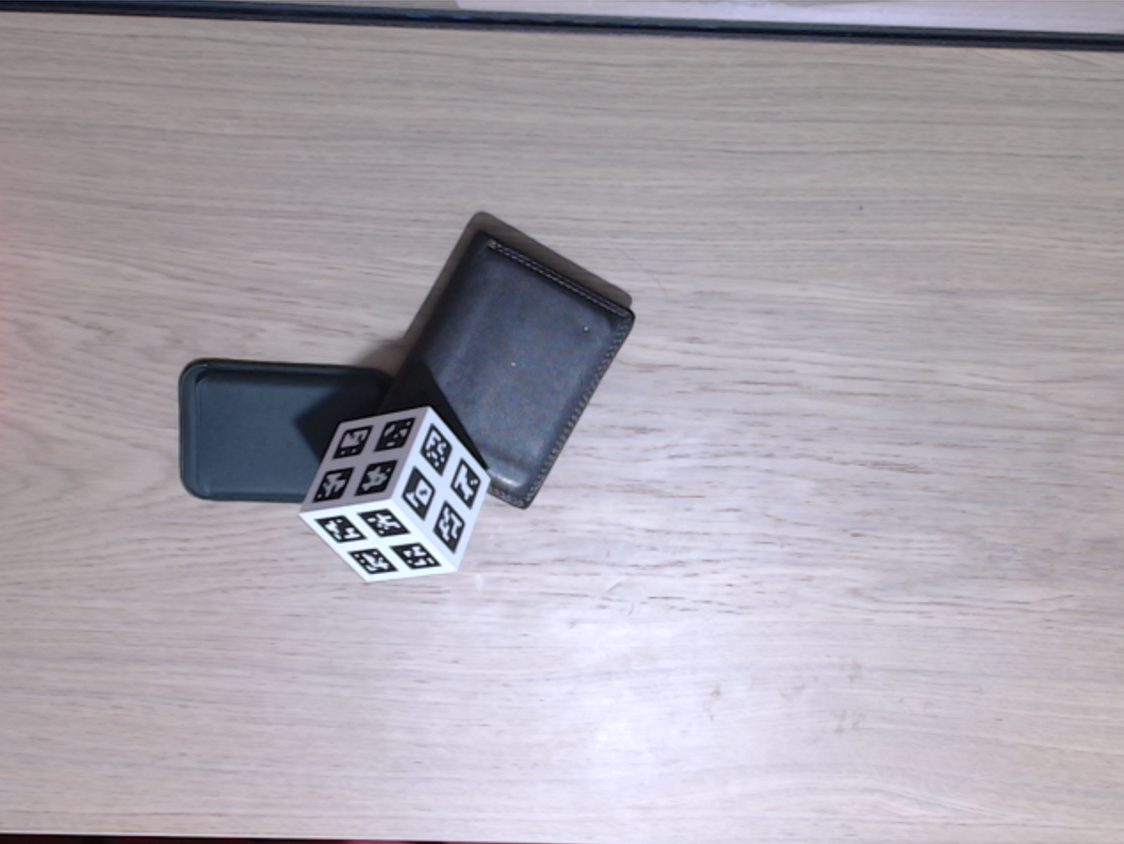
\includegraphics[width=0.8\textwidth]{imaxes/tilted_raw_image.png}
	\caption{Imagen original del marcador inclinado.}
	\label{fig:tilted_raw}
\end{figure}

\begin{figure}[H]
	\centering
	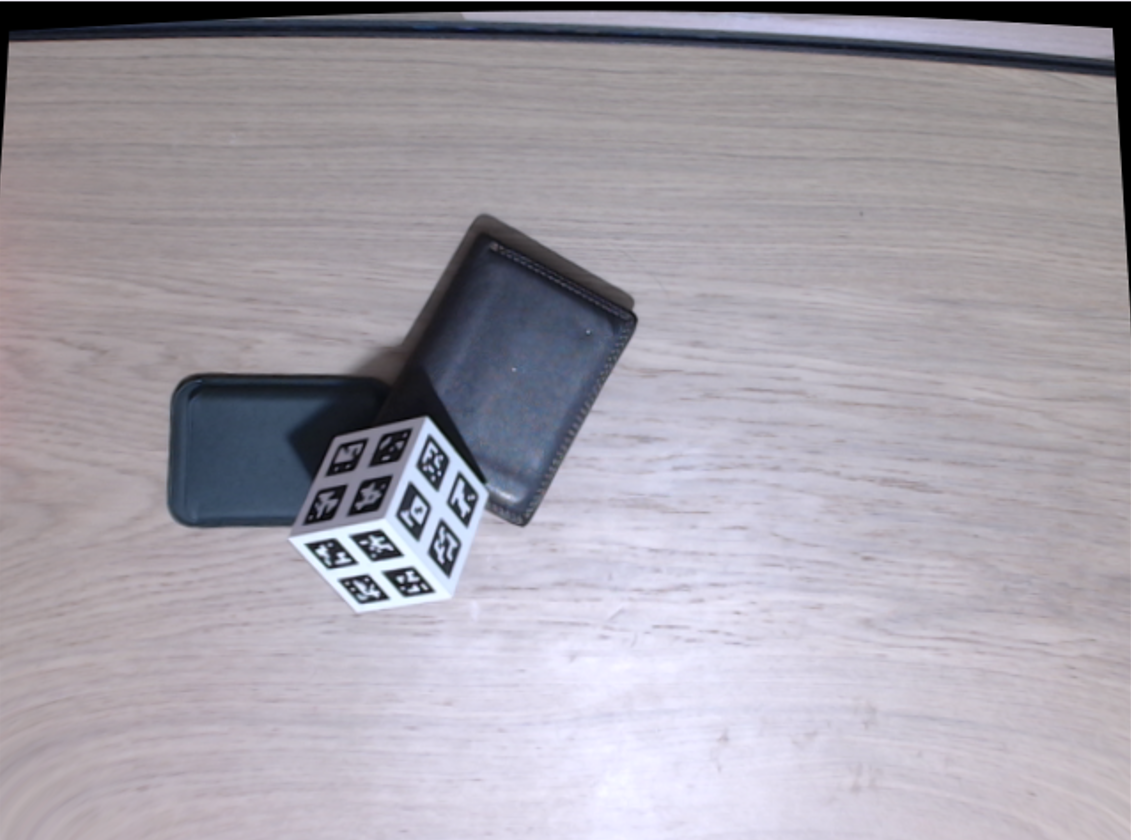
\includegraphics[width=0.8\textwidth]{imaxes/tilted_undistorted.png}
	\caption{Imagen corregida del marcador.}
	\label{fig:tilted_undistorted}
\end{figure}

\begin{figure}[H]
	\centering
	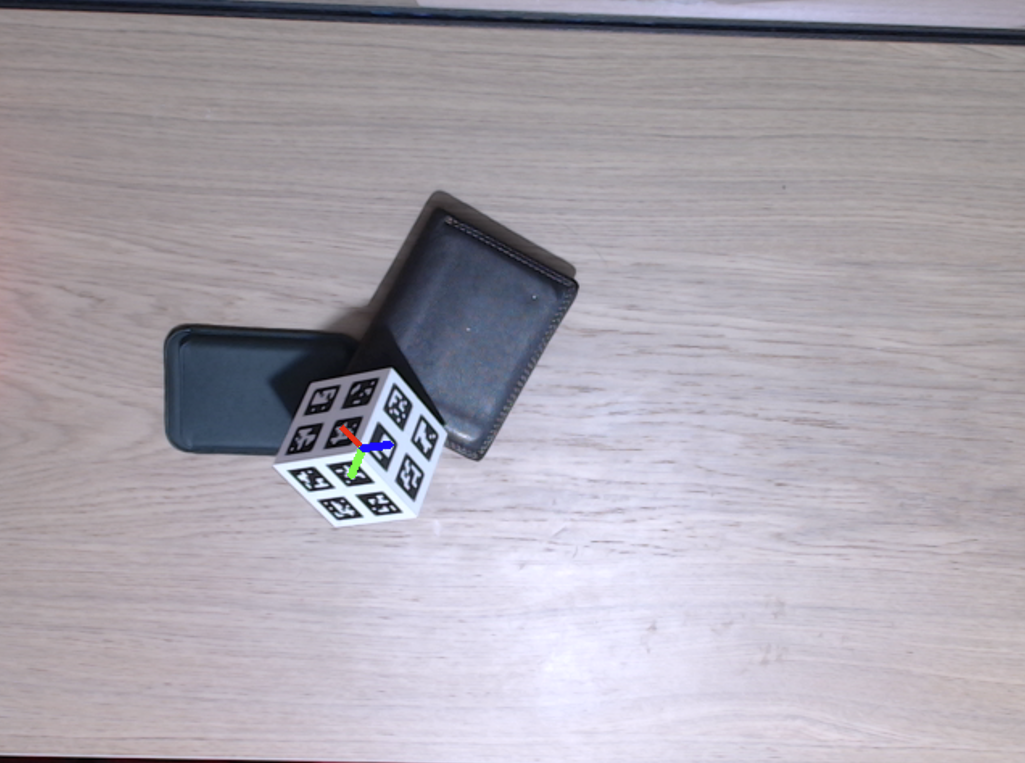
\includegraphics[width=0.8\textwidth]{imaxes/tilted_cube_axis.png}
	\caption{Ejes de coordenadas renderizados sobre el marcador.}
	\label{fig:tilted_axes}
\end{figure}

\begin{figure}[H]
	\centering
	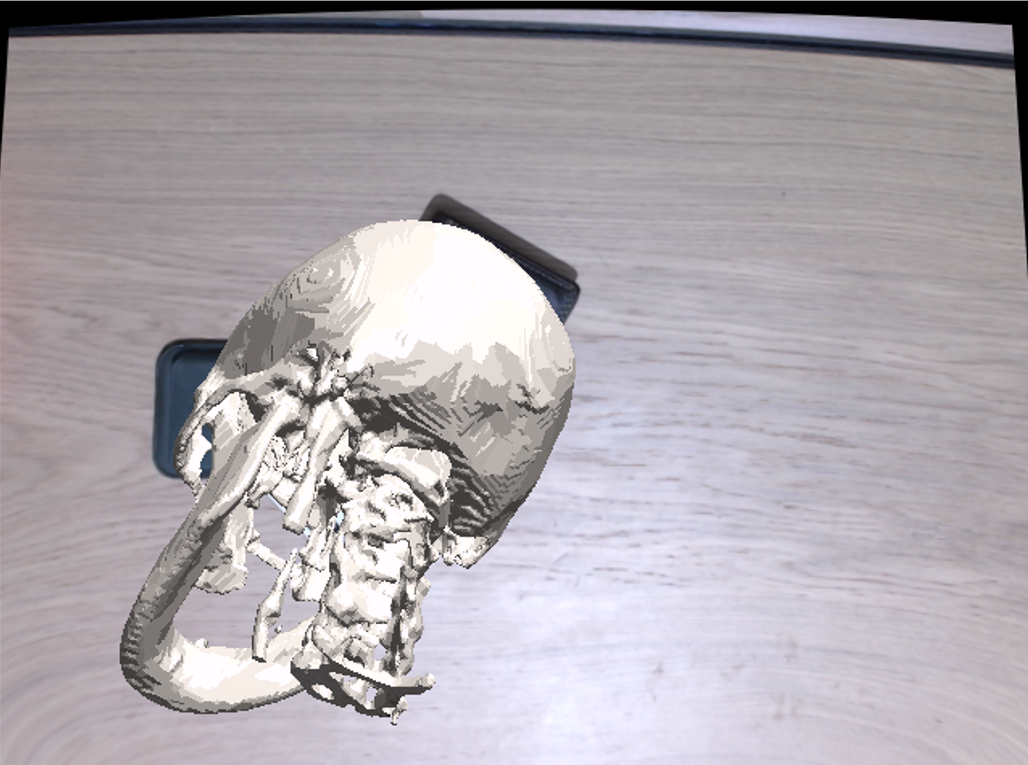
\includegraphics[width=0.8\textwidth]{imaxes/tilted_opengl_render.png}
	\caption{Modelo 3D renderizado sobre el marcador.}
	\label{fig:tilted_render}
\end{figure}

\section{Escenario con oclusión parcial}
\label{sec:ocluded}

En este escenario se evalúa la capacidad del sistema para mantener el seguimiento cuando parte del marcador cúbico está oculto.

\begin{figure}[H]
	\centering
	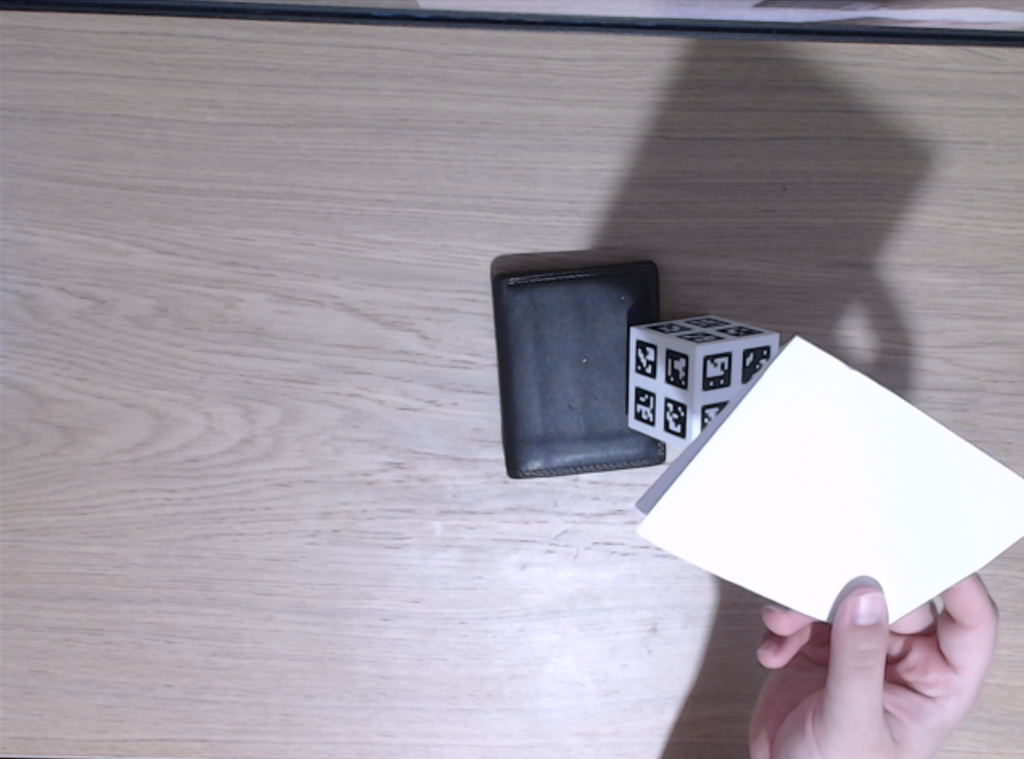
\includegraphics[width=0.8\textwidth]{imaxes/ocluded_raw_image.png}
	\caption{Imagen original del marcador con oclusión parcial.}
	\label{fig:ocluded_raw}
\end{figure}

\begin{figure}[H]
	\centering
	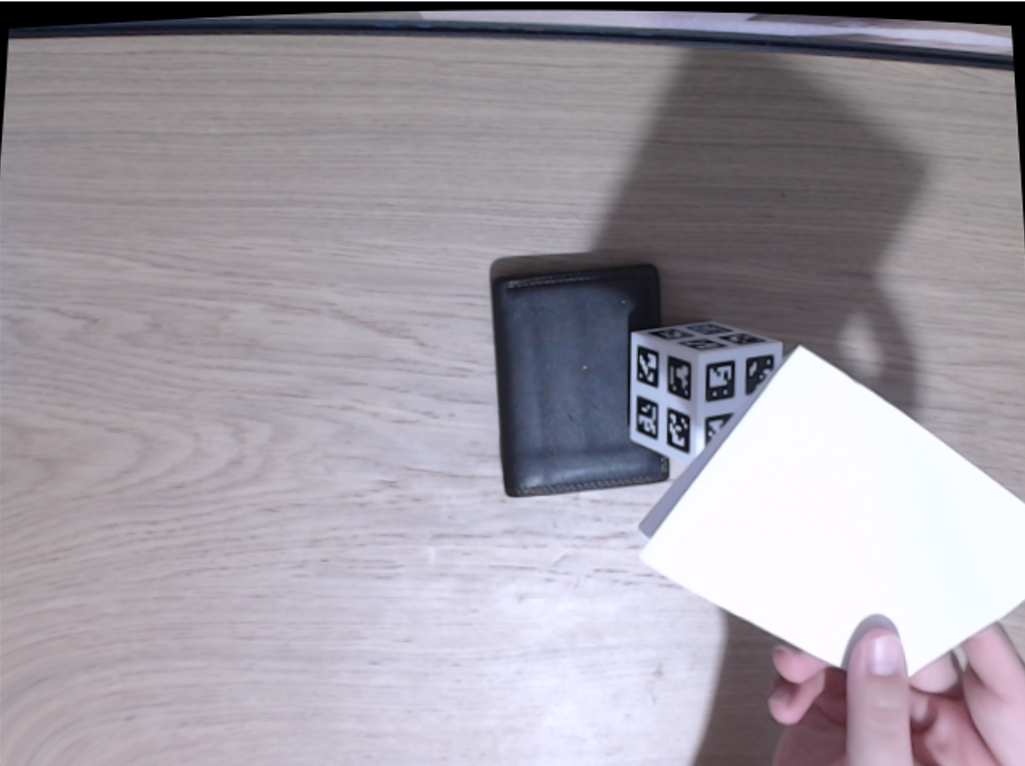
\includegraphics[width=0.8\textwidth]{imaxes/ocluded_undistorted.png}
	\caption{Imagen corregida del marcador ocluido tras la corrección de distorsión.}
	\label{fig:ocluded_undistorted}
\end{figure}

\begin{figure}[H]
	\centering
	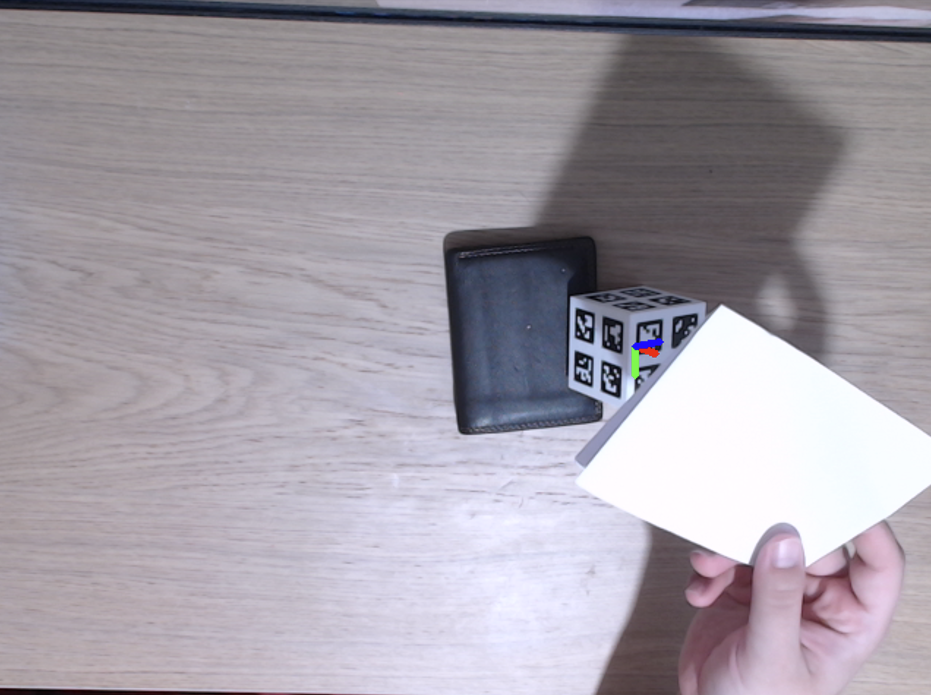
\includegraphics[width=0.8\textwidth]{imaxes/ocluded_cube_axis.png}
	\caption{Ejes de coordenadas renderizados sobre el marcador parcialmente ocluido.}
	\label{fig:ocluded_axes}
\end{figure}

\begin{figure}[H]
	\centering
	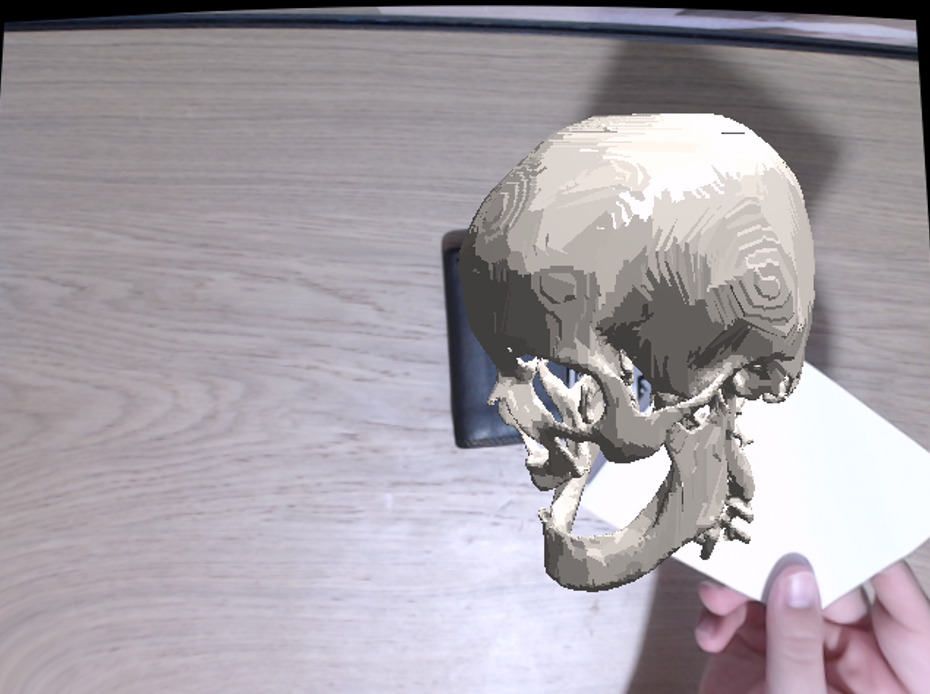
\includegraphics[width=0.8\textwidth]{imaxes/ocluded_opengl_render.png}
	\caption{Modelo 3D renderizado sobre el marcador.}
	\label{fig:ocluded_render}
\end{figure}

\printglossary[type=\acronymtype,title=\nomeglosarioacronimos]
\printglossary[title=\nomeglosariotermos]

\bibliographystyle{IEEEtranN}
\bibliography{\bibconfig,bibliografia/bibliografia}
\clearpage

\end{document}

%%%%%%%%%%%%%%%%%%%%%%%%%%%%%%%%%%%%%%%%%%%%%%%%%%%%%%%%%%%%%%%%%%%%%%%%%%%%%%%%
